\documentclass[10pt]{article}
%DIF LATEXDIFF DIFFERENCE FILE
%DIF DEL old.tex    Fri Dec  2 12:53:05 2022
%DIF ADD main.tex   Fri Dec  2 12:51:14 2022
\usepackage[utf8]{inputenc}
\usepackage[english]{babel}
\usepackage[font=small,labelfont=bf]{caption}
\usepackage{geometry}
\usepackage{natbib}
\usepackage{pxfonts}
\usepackage{graphicx}
% \graphicspath{ {./figures-low/} }
% \DeclareGraphicsExtensions{.png,.pdf}
\graphicspath{ {./figures-default/} }
\usepackage{newfloat}
\usepackage{setspace}
\usepackage{hyperref}
\usepackage{lineno}
\usepackage{placeins}
\usepackage{authblk}
\usepackage{textcomp}
\usepackage{listings}
%DIF 20a20-21
\usepackage[colorinlistoftodos]{todonotes} %DIF > 
\setuptodonotes{fancyline, inline} %DIF > 
%DIF -------
\hypersetup{
  colorlinks=true,
  citecolor=black,
  linkcolor=black,
  }
\bibliographystyle{apalike}
\doublespacing
\linenumbers

\title{The psychological arrow of time drives temporal asymmetries in retrodicting versus predicting narrative events}
\author[1]{Xinming Xu}
\author[2]{Ziyan Zhu}
\author[1, $\star$]{Jeremy R. Manning}
\affil[1]{Dartmouth College, Hanover, NH, USA}
\affil[2]{Peking University, Beijing, China}
\affil[$\star$]{Address correspondence to jeremy.r.manning@dartmouth.edu}

\newcommand{\stimDescription}{S1} % table
\newcommand{\segments}{S1} % figure
\newcommand{\events}{S2} %
\newcommand{\references}{S3}
%DIF PREAMBLE EXTENSION ADDED BY LATEXDIFF
%DIF UNDERLINE PREAMBLE %DIF PREAMBLE
\RequirePackage[normalem]{ulem} %DIF PREAMBLE
\RequirePackage{color}\definecolor{RED}{rgb}{1,0,0}\definecolor{BLUE}{rgb}{0,0,1} %DIF PREAMBLE
\providecommand{\DIFaddtex}[1]{{\protect\color{blue}\uwave{#1}}} %DIF PREAMBLE
\providecommand{\DIFdeltex}[1]{{\protect\color{red}\sout{#1}}}                      %DIF PREAMBLE
%DIF SAFE PREAMBLE %DIF PREAMBLE
\providecommand{\DIFaddbegin}{} %DIF PREAMBLE
\providecommand{\DIFaddend}{} %DIF PREAMBLE
\providecommand{\DIFdelbegin}{} %DIF PREAMBLE
\providecommand{\DIFdelend}{} %DIF PREAMBLE
\providecommand{\DIFmodbegin}{} %DIF PREAMBLE
\providecommand{\DIFmodend}{} %DIF PREAMBLE
%DIF FLOATSAFE PREAMBLE %DIF PREAMBLE
\providecommand{\DIFaddFL}[1]{\DIFadd{#1}} %DIF PREAMBLE
\providecommand{\DIFdelFL}[1]{\DIFdel{#1}} %DIF PREAMBLE
\providecommand{\DIFaddbeginFL}{} %DIF PREAMBLE
\providecommand{\DIFaddendFL}{} %DIF PREAMBLE
\providecommand{\DIFdelbeginFL}{} %DIF PREAMBLE
\providecommand{\DIFdelendFL}{} %DIF PREAMBLE
%DIF HYPERREF PREAMBLE %DIF PREAMBLE
\providecommand{\DIFadd}[1]{\texorpdfstring{\DIFaddtex{#1}}{#1}} %DIF PREAMBLE
\providecommand{\DIFdel}[1]{\texorpdfstring{\DIFdeltex{#1}}{}} %DIF PREAMBLE
\newcommand{\DIFscaledelfig}{0.5}
%DIF HIGHLIGHTGRAPHICS PREAMBLE %DIF PREAMBLE
\RequirePackage{settobox} %DIF PREAMBLE
\RequirePackage{letltxmacro} %DIF PREAMBLE
\newsavebox{\DIFdelgraphicsbox} %DIF PREAMBLE
\newlength{\DIFdelgraphicswidth} %DIF PREAMBLE
\newlength{\DIFdelgraphicsheight} %DIF PREAMBLE
% store original definition of \includegraphics %DIF PREAMBLE
\LetLtxMacro{\DIFOincludegraphics}{\includegraphics} %DIF PREAMBLE
\newcommand{\DIFaddincludegraphics}[2][]{{\color{blue}\fbox{\DIFOincludegraphics[#1]{#2}}}} %DIF PREAMBLE
\newcommand{\DIFdelincludegraphics}[2][]{% %DIF PREAMBLE
\sbox{\DIFdelgraphicsbox}{\DIFOincludegraphics[#1]{#2}}% %DIF PREAMBLE
\settoboxwidth{\DIFdelgraphicswidth}{\DIFdelgraphicsbox} %DIF PREAMBLE
\settoboxtotalheight{\DIFdelgraphicsheight}{\DIFdelgraphicsbox} %DIF PREAMBLE
\scalebox{\DIFscaledelfig}{% %DIF PREAMBLE
\parbox[b]{\DIFdelgraphicswidth}{\usebox{\DIFdelgraphicsbox}\\[-\baselineskip] \rule{\DIFdelgraphicswidth}{0em}}\llap{\resizebox{\DIFdelgraphicswidth}{\DIFdelgraphicsheight}{% %DIF PREAMBLE
\setlength{\unitlength}{\DIFdelgraphicswidth}% %DIF PREAMBLE
\begin{picture}(1,1)% %DIF PREAMBLE
\thicklines\linethickness{2pt} %DIF PREAMBLE
{\color[rgb]{1,0,0}\put(0,0){\framebox(1,1){}}}% %DIF PREAMBLE
{\color[rgb]{1,0,0}\put(0,0){\line( 1,1){1}}}% %DIF PREAMBLE
{\color[rgb]{1,0,0}\put(0,1){\line(1,-1){1}}}% %DIF PREAMBLE
\end{picture}% %DIF PREAMBLE
}\hspace*{3pt}}} %DIF PREAMBLE
} %DIF PREAMBLE
\LetLtxMacro{\DIFOaddbegin}{\DIFaddbegin} %DIF PREAMBLE
\LetLtxMacro{\DIFOaddend}{\DIFaddend} %DIF PREAMBLE
\LetLtxMacro{\DIFOdelbegin}{\DIFdelbegin} %DIF PREAMBLE
\LetLtxMacro{\DIFOdelend}{\DIFdelend} %DIF PREAMBLE
\DeclareRobustCommand{\DIFaddbegin}{\DIFOaddbegin \let\includegraphics\DIFaddincludegraphics} %DIF PREAMBLE
\DeclareRobustCommand{\DIFaddend}{\DIFOaddend \let\includegraphics\DIFOincludegraphics} %DIF PREAMBLE
\DeclareRobustCommand{\DIFdelbegin}{\DIFOdelbegin \let\includegraphics\DIFdelincludegraphics} %DIF PREAMBLE
\DeclareRobustCommand{\DIFdelend}{\DIFOaddend \let\includegraphics\DIFOincludegraphics} %DIF PREAMBLE
\LetLtxMacro{\DIFOaddbeginFL}{\DIFaddbeginFL} %DIF PREAMBLE
\LetLtxMacro{\DIFOaddendFL}{\DIFaddendFL} %DIF PREAMBLE
\LetLtxMacro{\DIFOdelbeginFL}{\DIFdelbeginFL} %DIF PREAMBLE
\LetLtxMacro{\DIFOdelendFL}{\DIFdelendFL} %DIF PREAMBLE
\DeclareRobustCommand{\DIFaddbeginFL}{\DIFOaddbeginFL \let\includegraphics\DIFaddincludegraphics} %DIF PREAMBLE
\DeclareRobustCommand{\DIFaddendFL}{\DIFOaddendFL \let\includegraphics\DIFOincludegraphics} %DIF PREAMBLE
\DeclareRobustCommand{\DIFdelbeginFL}{\DIFOdelbeginFL \let\includegraphics\DIFdelincludegraphics} %DIF PREAMBLE
\DeclareRobustCommand{\DIFdelendFL}{\DIFOaddendFL \let\includegraphics\DIFOincludegraphics} %DIF PREAMBLE
%DIF COLORLISTINGS PREAMBLE %DIF PREAMBLE
\RequirePackage{listings} %DIF PREAMBLE
\RequirePackage{color} %DIF PREAMBLE
\lstdefinelanguage{DIFcode}{ %DIF PREAMBLE
%DIF DIFCODE_UNDERLINE %DIF PREAMBLE
  moredelim=[il][\color{red}\sout]{\%DIF\ <\ }, %DIF PREAMBLE
  moredelim=[il][\color{blue}\uwave]{\%DIF\ >\ } %DIF PREAMBLE
} %DIF PREAMBLE
\lstdefinestyle{DIFverbatimstyle}{ %DIF PREAMBLE
	language=DIFcode, %DIF PREAMBLE
	basicstyle=\ttfamily, %DIF PREAMBLE
	columns=fullflexible, %DIF PREAMBLE
	keepspaces=true %DIF PREAMBLE
} %DIF PREAMBLE
\lstnewenvironment{DIFverbatim}{\lstset{style=DIFverbatimstyle}}{} %DIF PREAMBLE
\lstnewenvironment{DIFverbatim*}{\lstset{style=DIFverbatimstyle,showspaces=true}}{} %DIF PREAMBLE
%DIF END PREAMBLE EXTENSION ADDED BY LATEXDIFF

\begin{document}

\maketitle

\begin{abstract}
\DIFdelbegin \DIFdel{Phenomena in classical physics are time-symmetric}\DIFdelend \DIFaddbegin \DIFadd{Statistical sequences are generally symmetric in time}\DIFaddend : given the present, \DIFdelbegin \DIFdel{physical systems’ }\DIFdelend \DIFaddbegin \DIFadd{the }\DIFaddend pasts and futures are equally knowable.  However, our knowledge about our own lives is time-asymmetric, since we remember our past, but not our future. When both the past and future are unobserved, as in \textit{other} people's lives, are our inferences about the past and future time-symmetric or asymmetric?  To study these questions, we had participants view segments of a character-driven television drama.  They used free-form responses to either retrodict what happened just prior, or predict what would happen next, relative to each just-watched segment. We found that participants' inferences were time-asymmetric, in that their retrodictions of past events were better than their predictions of the future. This asymmetry was driven by characters' biases in conversational references to their own pasts.  Our work reveals a temporal asymmetry in how observations of other humans’ behaviors inform us about the past versus future.
\end{abstract}


\section*{Introduction}
\DIFdelbegin \DIFdel{How do we conceptualize the past and future?  Because we have memories of our past (but not our future), we have asymmetric information in the present about our own past versus our own future.  This is referred to as the psychological arrow of time~\mbox{%DIFAUXCMD
\citep[e.g.,][]{Hawk85}}\hskip0pt%DIFAUXCMD
.
Memories must refer to the past, but not all events that happened in the past are encoded into memories. This is especially true when we estimate the pasts and futures of }\textit{\DIFdel{other}} %DIFAUXCMD
\DIFdel{people's lives, e.g., when we may be equally ignorant of }\DIFdelend \DIFaddbegin 

\DIFadd{Life unfolds over time. For every moment, we only have direct access to }\DIFaddend the \DIFaddbegin \DIFadd{current state of the world. To what extent can the current state tells us about the }\DIFaddend past and\DIFdelbegin \DIFdel{future relative to a given moment.
}\DIFdelend \DIFaddbegin \DIFadd{/or the future? 
One way of examining this question is to look at highly simplified sequences that are artificially constructed in the laboratory \mbox{%DIFAUXCMD
\citep[e.g., ][]{MaheEtal22}}\hskip0pt%DIFAUXCMD
. 
At one extreme, for deterministic sequences, once the rules generating the sequences are learned, observing the current state provides sufficient information to reconstruct the entire past and future history of the stimulus. 
At another extreme, for random sequences, observing the current state provides no information about the past or future.
}\DIFaddend 

\DIFdelbegin \DIFdel{When we interact with other people, we experience (and, potentially, encode) the present of other people's lives.  We may predict what is likely to happen in their future~\mbox{%DIFAUXCMD
\citep{TamiThor18, KostSaxe13}}\hskip0pt%DIFAUXCMD
, or draw inferences about what happened in their past.  These estimates can draw on events that unfold over a variety of timescales.  For example, when we use contextual cues to join an in-progress conversation, we might draw on a brief phrase we happened to overhear a moment ago, or we might draw on knowledge acquired over a lifetime of friendship with one of the individuals who is conversing.  In turn, we can use this information to form estimates at different timescales.  This could include guessing about what topics the conversation might have covered (or proceed to cover) in the immediate past or future, or about events in the other participants' lives that occurred (or will occur) in the distant past or future. 
In contrast to prediction, we refer to the act of inferring the unobserved past as }\textit{\DIFdel{retrodiction}} %DIFAUXCMD
\DIFdel{(Fig.~\ref{fig:intro1}). Relative to prediction (i.e., the act of estimating or inferring the future), retrodiction (or postdiction) has been relatively under-studied~\mbox{%DIFAUXCMD
\citep[but see, e.g.,][]{EaglSejn00}}\hskip0pt%DIFAUXCMD
.  Here we seek to elucidate the symmetries and asymmetries in how accurately we are able to retrodict the unobserved past versus predict the unobserved future }\DIFdelend \DIFaddbegin \DIFadd{Sequences generated by stochastic processes are between these two extremes. One typical example is sequences generated by Markov processes, whereby each state in the sequence is solely dependent on the immediately preceding state}\DIFaddend . \DIFdelbegin \DIFdel{For example, are retrodiction and prediction time-symmetric?   Or, if we only observe the present of other people's lives, are we likely to know more about their pasts, or more about their futures?
}%DIFDELCMD < 

%DIFDELCMD < \begin{figure}[tp]
%DIFDELCMD <   \centering
%DIFDELCMD <   \includegraphics[width=\textwidth]{intro1}
%DIFDELCMD <   %%%
%DIFDELCMD < \caption{%
{%DIFAUXCMD
\textbf{\DIFdelFL{Retrodiction, retrospection, and prediction.}} %DIFAUXCMD
\DIFdelFL{In one's own life, one may draw on memory to retrospect (i.e., review or re-evaluate) the past and/or predict the future.  This process is time-asymmetric, since our own past is (typically) observed whereas our future is not.  When we make inferences about }\textit{\DIFdelFL{other}} %DIFAUXCMD
\DIFdelFL{people's lives, however, we often have uncertainty about both their past and future, since we may have observed neither.  We may }\textit{\DIFdelFL{retrodict}} %DIFAUXCMD
\DIFdelFL{the unobserved past and predict the unobserved future of other people's lives.}}
  %DIFAUXCMD
%DIFDELCMD < \label{fig:intro1}
%DIFDELCMD < \end{figure}
%DIFDELCMD < 

%DIFDELCMD < %%%
\DIFdel{Laws from classical physics are time-symmetric. For example , given the measurements of the position and velocity of an object, we are able to perfectly calculate its past stateas well as its future state, both of which are deterministic. In stochastic (non-deterministic) systems, we can draw on information theory to ask whether the present contains the same amount of mutual information about the preceding (past ) and proceeding (future ) states .  In other words, does }\DIFdelend \DIFaddbegin \DIFadd{For such probabilistic sequences, Shannon entropy can be used to quantify the uncertainty of the past states or the future states given the current state. 
While the exact level of uncertainty varies for processes with different statistical structures, here, we are interested in whether there is a time-symmetry such that }\DIFaddend knowing the present \DIFdelbegin \DIFdel{reduce uncertainty about }\DIFdelend \DIFaddbegin \DIFadd{reduces the uncertainty of }\DIFaddend the past and \DIFaddbegin \DIFadd{the }\DIFaddend future to the same \DIFdelbegin \DIFdel{degree?  }\DIFdelend \DIFaddbegin \DIFadd{amount.
}\DIFaddend \cite{Cove94} showed that, for any stationary process (i.e., processes in equilibrium), Markov or otherwise, the present state shares the same amount of mutual information with the past state and future state~\citep[also see][]{BialEtal01, ElliEtal09}. Further, there is some evidence that humans perform similarly when attempting to estimate the previous or next item in sequences governed by stochastic Markov processes~\citep{JonePash07}. 

\DIFaddbegin \begin{figure}[tp]
  \centering
  \includegraphics[width=\textwidth]{intro1}
  \caption{\textbf{\DIFaddFL{Retrodiction, retrospection, and prediction.}} \DIFaddFL{In one's own life, one may draw on memory to retrospect (i.e., review or re-evaluate) the past and/or predict the future.  This process is time-asymmetric, since our own past is (typically) observed whereas our future is not.  When we make inferences about }\textit{\DIFaddFL{other}} \DIFaddFL{people's lives, however, we often have uncertainty about both their past and future, since we may have observed neither.  We may }\textit{\DIFaddFL{retrodict}} \DIFaddFL{the unobserved past and predict the unobserved future of other people's lives.}}
  \label{fig:intro1}
\end{figure}

\DIFaddend Does time-symmetry also hold for real-world experiences and events? \DIFaddbegin \DIFadd{In other words, given the present, can we tell the future and the past equally well?
For real life, there seem to be fundamental differences between the past and the future. For example, we have memories of our past, but not our future. This is referred to as the psychological arrow of time~\mbox{%DIFAUXCMD
\citep[e.g.,][]{Hawk85}}\hskip0pt%DIFAUXCMD
. This results in our knowledge-asymmetry of the past and the future. Besides, we have some volitional control of our future, but not our past. 
Since our memories in the present reflect past experiences, we are trivially able to “infer” what happened in the past. On the other hand, since we have some volitional control of future experiences, we may also be trivially able to "infer" what will happen in the future (by leveraging our volitional control).
}

\DIFadd{Suppose, however, that we were to encounter a real-world scenario where we were equally ignorant of the past and future. For example, suppose we saw a stranger for the first time. In this scenario, we observe (and, potentially, encode) the present of the stranger's life, we may predict what is likely to happen in their future~\mbox{%DIFAUXCMD
\citep{TamiThor18, KostSaxe13}}\hskip0pt%DIFAUXCMD
, or draw inferences about what happened in their past. In contrast to prediction, we refer to the act of inferring the unobserved past as }\textit{\DIFadd{retrodiction}} \DIFadd{(Fig.~\ref{fig:intro1}). 
In general, when we observe only the present and the past and future are both unobserved, are we better at retrodicting the past or predicting the future?
}

\DIFadd{Now let's consider what are the ways we can retrodict the past and predict the future based on observation of the present.
}\DIFaddend Imagine that you have been living in City A for your entire life, and you are visiting City B for the first time.  How might you guess at what yesterday's weather might have been in City B (Fig.~\ref{fig:intro2}A)?  Perhaps you might draw on statistical regularities in weather patterns you observed in City A-- for example sunny or warm weather today could suggest that yesterday and tomorrow might also be sunny and warm.  Drawing solely on learned \DIFdelbegin \DIFdel{transition probabilities }\DIFdelend \DIFaddbegin \DIFadd{statistical regularities }\DIFaddend between different weather patterns, you would have roughly equal information about yesterday's and tomorrow's weather in City B, conditioned on the weather you observe today.

\begin{figure}[tp]
  \centering
  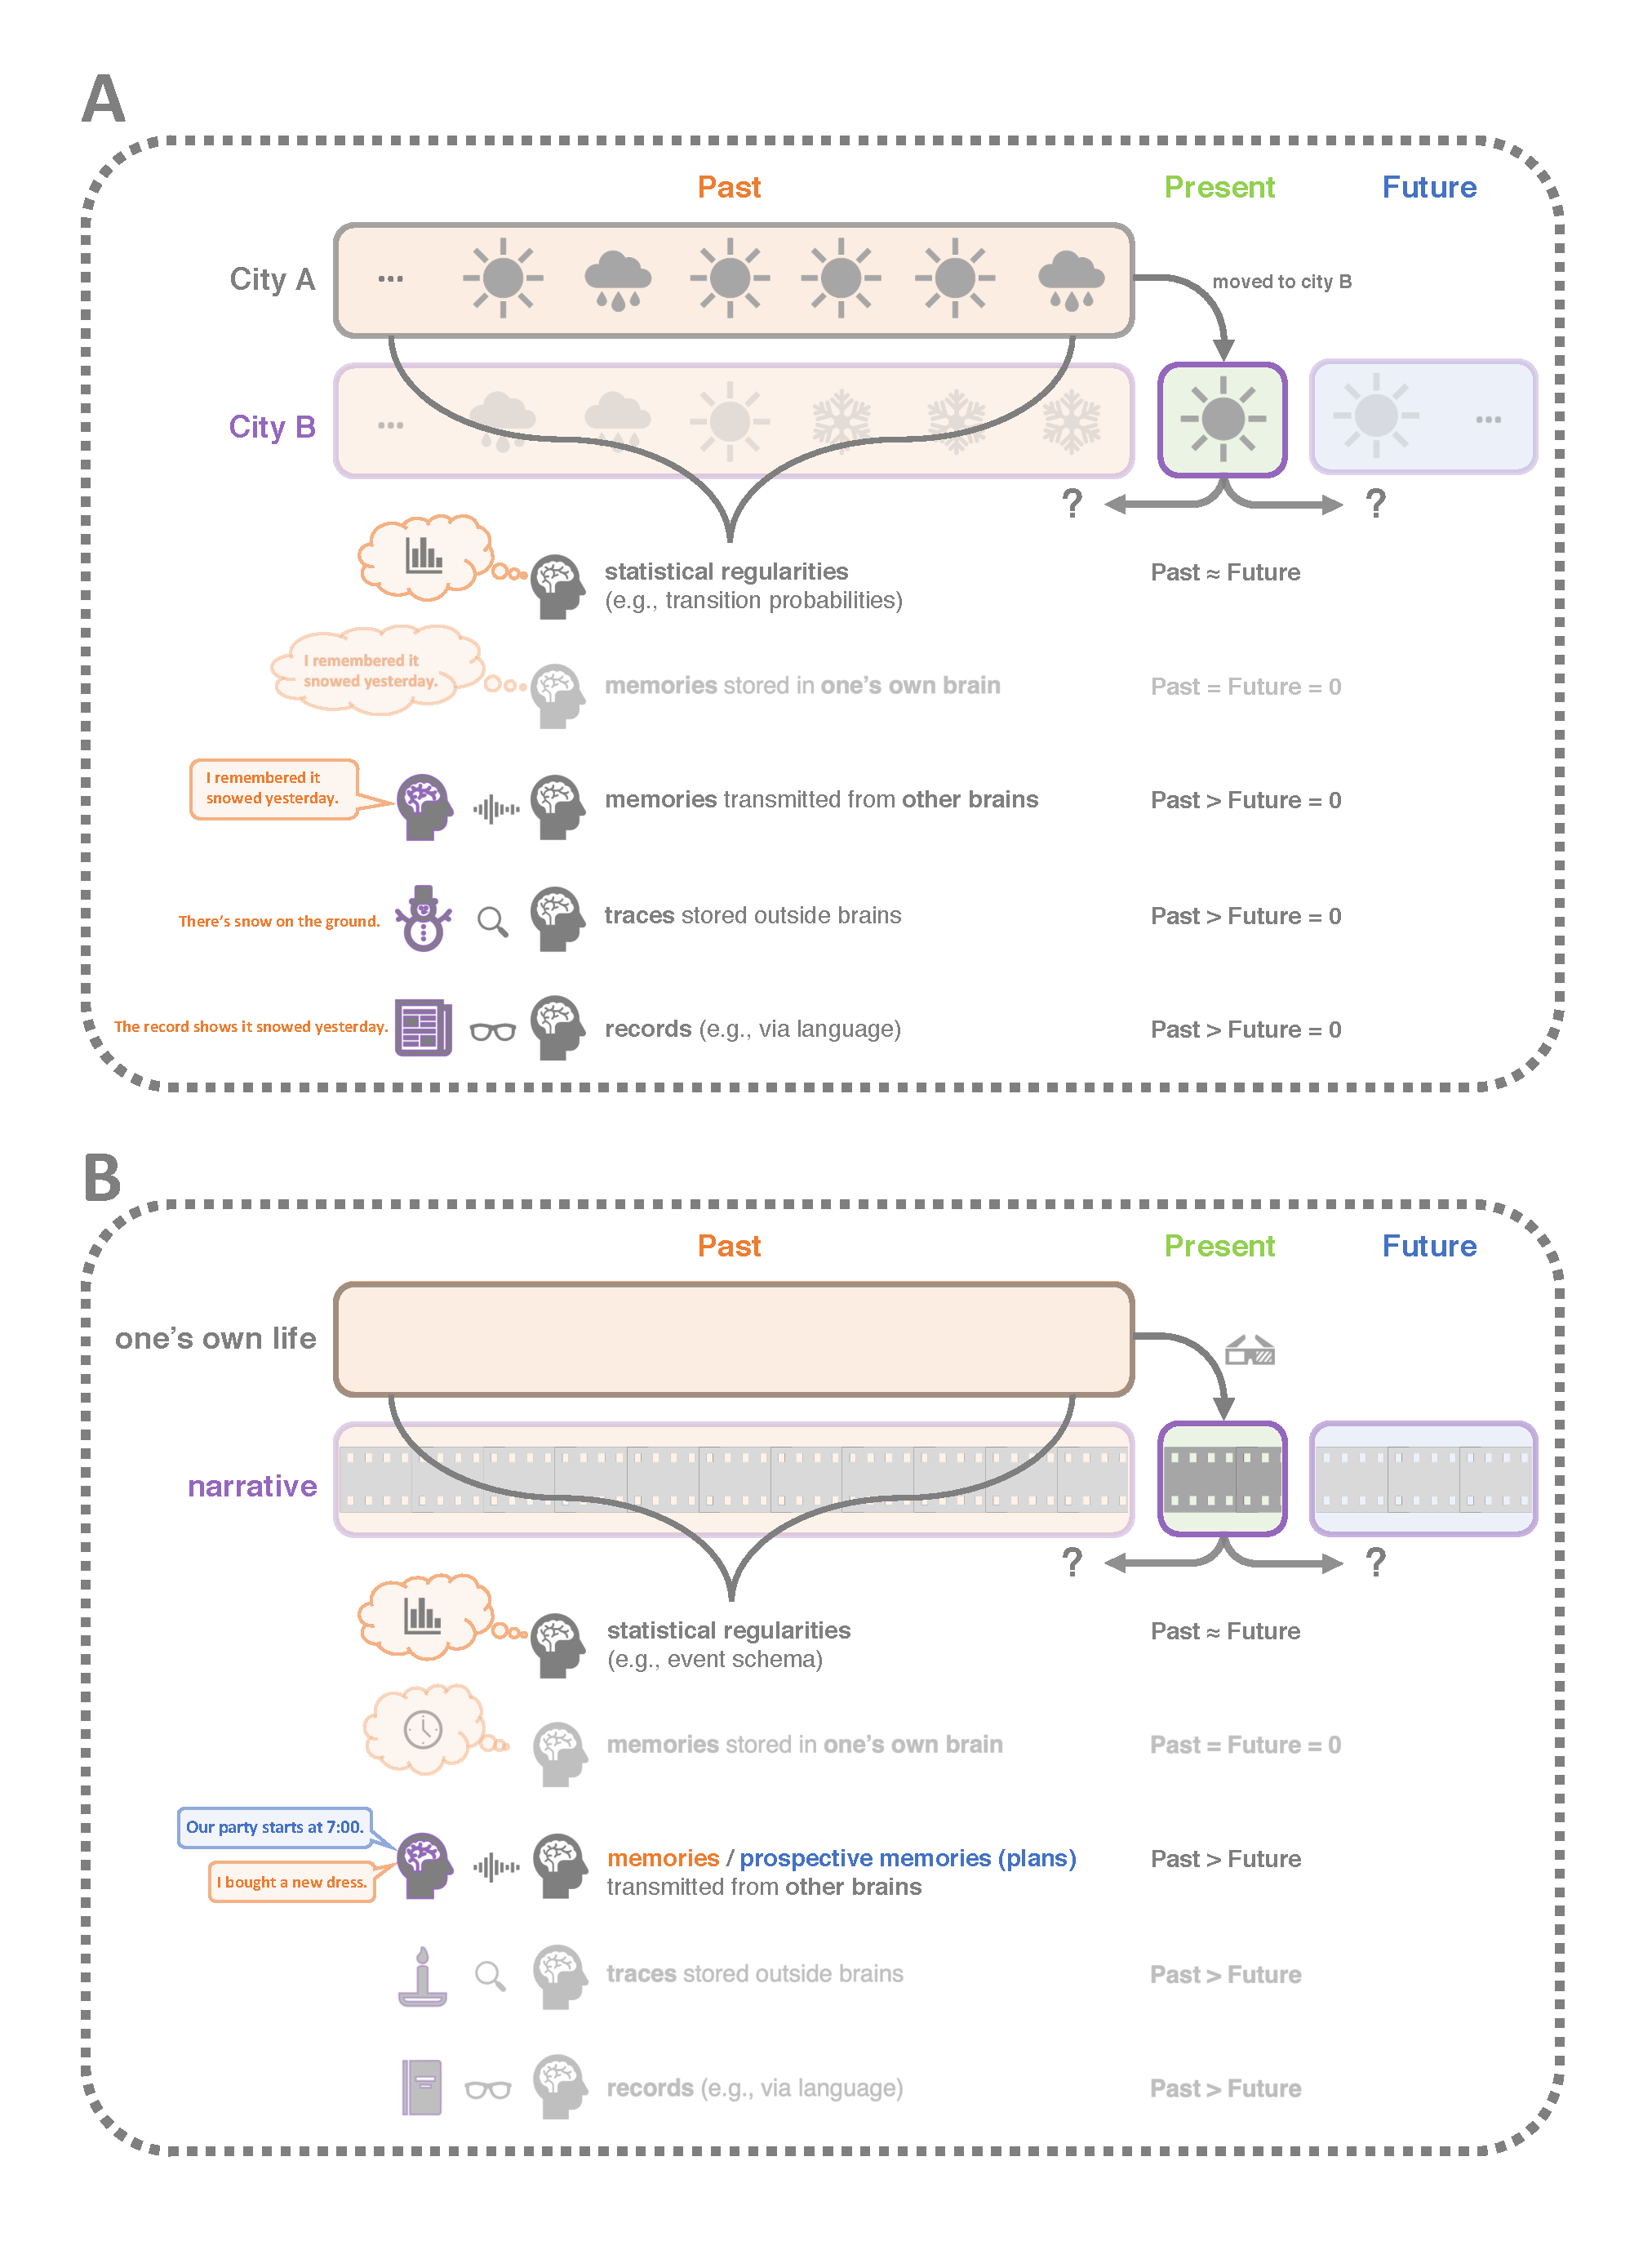
\includegraphics[width=.65\textwidth]{intro2}
\vspace{-0.2in}
  \caption{ \textbf{The many ways to know about the past and the future.} \textbf{A.}
    Suppose you are from City A, and you are visiting City B for the first time.  To retrodict what City B's weather might have been yesterday, you might draw on learned statistical regularities (e.g., experienced in City A), memories stored in other people's brains, traces stored outside of brains, and records.  Note that you could not draw on your own memories, since you did not experience yesterday's weather in City B.  Predicting City B's weather tomorrow can draw only on statistical regularities, since no direct traces of tomorrow's weather occur in the present.  (For example, clouds may gather before a snow storm, but memories of snow and traces of snow on the ground will not appear until it begins to fall.)   \textbf{B.}  If you start watching a movie from the halfway point, you might draw on information gleaned from the current scene to retrodict what had happened previously or predict what might happen next.  Unlike in your own life, however, your memories would not directly inform you about the past.  Nor could you interact with the environment to gather additional relevant information or examine historical records outside of the scope of the narrative.  Rather, your retrodictions and predictions about other parts of the movie might draw on statistical regularities learned from your other life experiences (e.g., schema knowledge).  We expect that inferences drawn from statistical regularities should be relatively symmetric (i.e., roughly equally informative about the past and future).  The characters' memories or prospective memories referenced in conversations might also inform you about what happened in the past or might happen in the future.}
  \label{fig:intro2}
\end{figure}

Although learned statistical regularities can provide relatively time-symmetric clues about the unobserved past and future, we can draw on additional clues that are time-asymmetric\DIFaddbegin \DIFadd{, that is, traces and records of the past (but not of the future) stored in the present}\DIFaddend . For example, since residents of City B might \DIFdelbegin \DIFdel{remember }\DIFdelend \DIFaddbegin \DIFadd{have memories of }\DIFaddend yesterday's weather (but not tomorrow's weather), observing a City B resident discussing yesterday's weather might provide a reliable answer. 
Observing City B residents might also provide indirect (non-verbal) hints.
Traces of yesterday's weather may also be observed in the broader environment (e.g., fresh snow on the ground) or in records (e.g., a newspaper's weather report from the previous day).  Each of these time-asymmetric sources provides more information about the past (yesterday's weather) than the future (tomorrow's weather).  Across all time-symmetric and time-asymmetric sources of information about the past and future, we generally have more information about the past.

In real-world experiences, and to an extent also in narratives (e.g., stories, movies, etc.), \DIFdelbegin \DIFdel{links between different events form a complex network.  For example, a }\DIFdelend \DIFaddbegin \DIFadd{the past, present, and future are also interdependent. A }\DIFaddend given moment in a movie may provide insight into what happened in the past or clues about what might happen in the future (Fig.~\ref{fig:intro2}B). Just as in the above weather retrodiction and prediction example, \DIFdelbegin \DIFdel{statistical regularities (e.g., event schema) }\DIFdelend \DIFaddbegin \DIFadd{in real-world experiences, there are also statistical regularities, for example, event schemas or scripts~\mbox{%DIFAUXCMD
\citep{BoweEtal79}}\hskip0pt%DIFAUXCMD
, which should }\DIFaddend provide roughly time-symmetric clues about the past and future (given the present).

\DIFdelbegin \DIFdel{In character-driven narratives, the ways characters behave, think, and interact can also provide information about past and future events in the narrative.  }\DIFdelend Because characters in narratives (like real-world people) are typically depicted as remembering their own pasts (but not their futures), narrative characters typically exhibit a psychological arrow of time reminiscent of real-world human experience.  In this way, observable clues from narrative characters~\citep[such as vicarious memories referenced in conversations;][]{PillEtal15}, and environmental cues all tend favor the past. \DIFdelbegin \DIFdel{Despite this asymmetry, narratives often provide }\textit{\DIFdel{some}} %DIFAUXCMD
\DIFdel{clues about what will happen in the future.  In addition to direct foreshadowing, characters might also }\DIFdelend \DIFaddbegin \DIFadd{On the other hand, characters in narratives are also typically depicted as having volitional control over their futures (but not their pasts), and characters might }\DIFaddend discuss or refer to their future plans. \DIFdelbegin \DIFdel{Because characters in a narrative (and people more generally) have control over their future behaviors and activities}\DIFdelend \DIFaddbegin \DIFadd{Thus}\DIFaddend , observing other people's behaviors in the present can provide information about their future beyond statistical regularities alone.  
\DIFdelbegin \DIFdel{This implies that temporal asymmetries in how much information we have about the past versus the future may depend in part on volitional control. In other words, when someone says they will take a particular action one month from now, this might provide more reliable information than that individual's prediction about what weather patterns would be observed one month from now.
}%DIFDELCMD < 

%DIFDELCMD < %%%
\DIFdel{Although there are many differences between }\DIFdelend \DIFaddbegin 

\DIFadd{In the current study, we used narratives as materials to study how we tell the past and the future from the present.
Although narratives differ from }\DIFaddend real-world \DIFdelbegin \DIFdel{events and narrative events, narratives }\DIFdelend \DIFaddbegin \DIFadd{evens in many ways, they }\DIFaddend often draw in the audience by attempting to evoke a sense of plausibility. As a consequence, narrative events, character behaviors, and character interactions often \DIFdelbegin \DIFdel{display a range of content, temporal associations, and causal relations, that are }\DIFdelend \DIFaddbegin \DIFadd{follow a believable structure that is }\DIFaddend reminiscent of real-world \DIFdelbegin \DIFdel{events. 
This can provide an interesting and useful medium for studying how people retrodict }\DIFdelend \DIFaddbegin \DIFadd{experiences. 
We designed a novel paradigm for exposing participants to scenarios where }\DIFaddend the past and \DIFdelbegin \DIFdel{predict the future .  In our study, we }\DIFdelend \DIFaddbegin \DIFadd{future could both be unobserved.
We }\DIFaddend asked participants to watch segments (movie clips) drawn from a \DIFaddbegin \DIFadd{character-driven dramatic }\DIFaddend television show, 
\DIFdelbegin \DIFdel{and to retrodict, predict, or recall different events}\DIFdelend \DIFaddbegin \DIFadd{The segments were chosen (and ordered) to control for how much of the past or future of the narrative participants had experienced before viewing the target segment.
Then we asked the participants to guess about what might have happened before the target segment (retrodiction), or what might happen after the target segment (prediction), or to recount what they had observed in the target segment (recall)}\DIFaddend .
We used human annotations and sentence-level natural language processing models to evaluate the quality of participants' retrodictions and predictions.  To foreshadow our results, we found that participants were overall better at retrodicting the past than predicting the future. This appeared to be driven by two main factors.  First, characters more often referred to past events than future (e.g., planned) events, and this influenced participants' responses. Second, associations and dependencies between temporally adjacent events enabled participants to form estimates about nearby events (e.g., to a just-watched scene or a past or future event referenced in an observed conversation).  Taken together, our work reveals a temporal asymmetry in how observations of other humans’ behaviors inform us about the past versus future.

\section*{Results}
Participants in our study ($n = 36$) watched segments from two storylines, drawn from the CBS television show, \textit{Why Women Kill}.  Each storyline comprised 11 segments (mean duration: 2.05~min; range: 0.97--3.87~min, Table \stimDescription).  We asked participants to use free-form (typed) text responses to retrodict what had happened prior to a just-watched segment, predict what would happen next, or recall what they had just watched. We referred to the to-be-retrodicted, to-be-predicted, or to-be-recalled segment as the target segment for each response. We systematically varied whether participants watched the segments in forward or reverse chronological order, and how many segments preceded or proceeded the target segment they had seen prior to making a response (Fig.~\ref{fig:method}, \textit{Task design}).

\begin{figure}[tp]
  \centering
  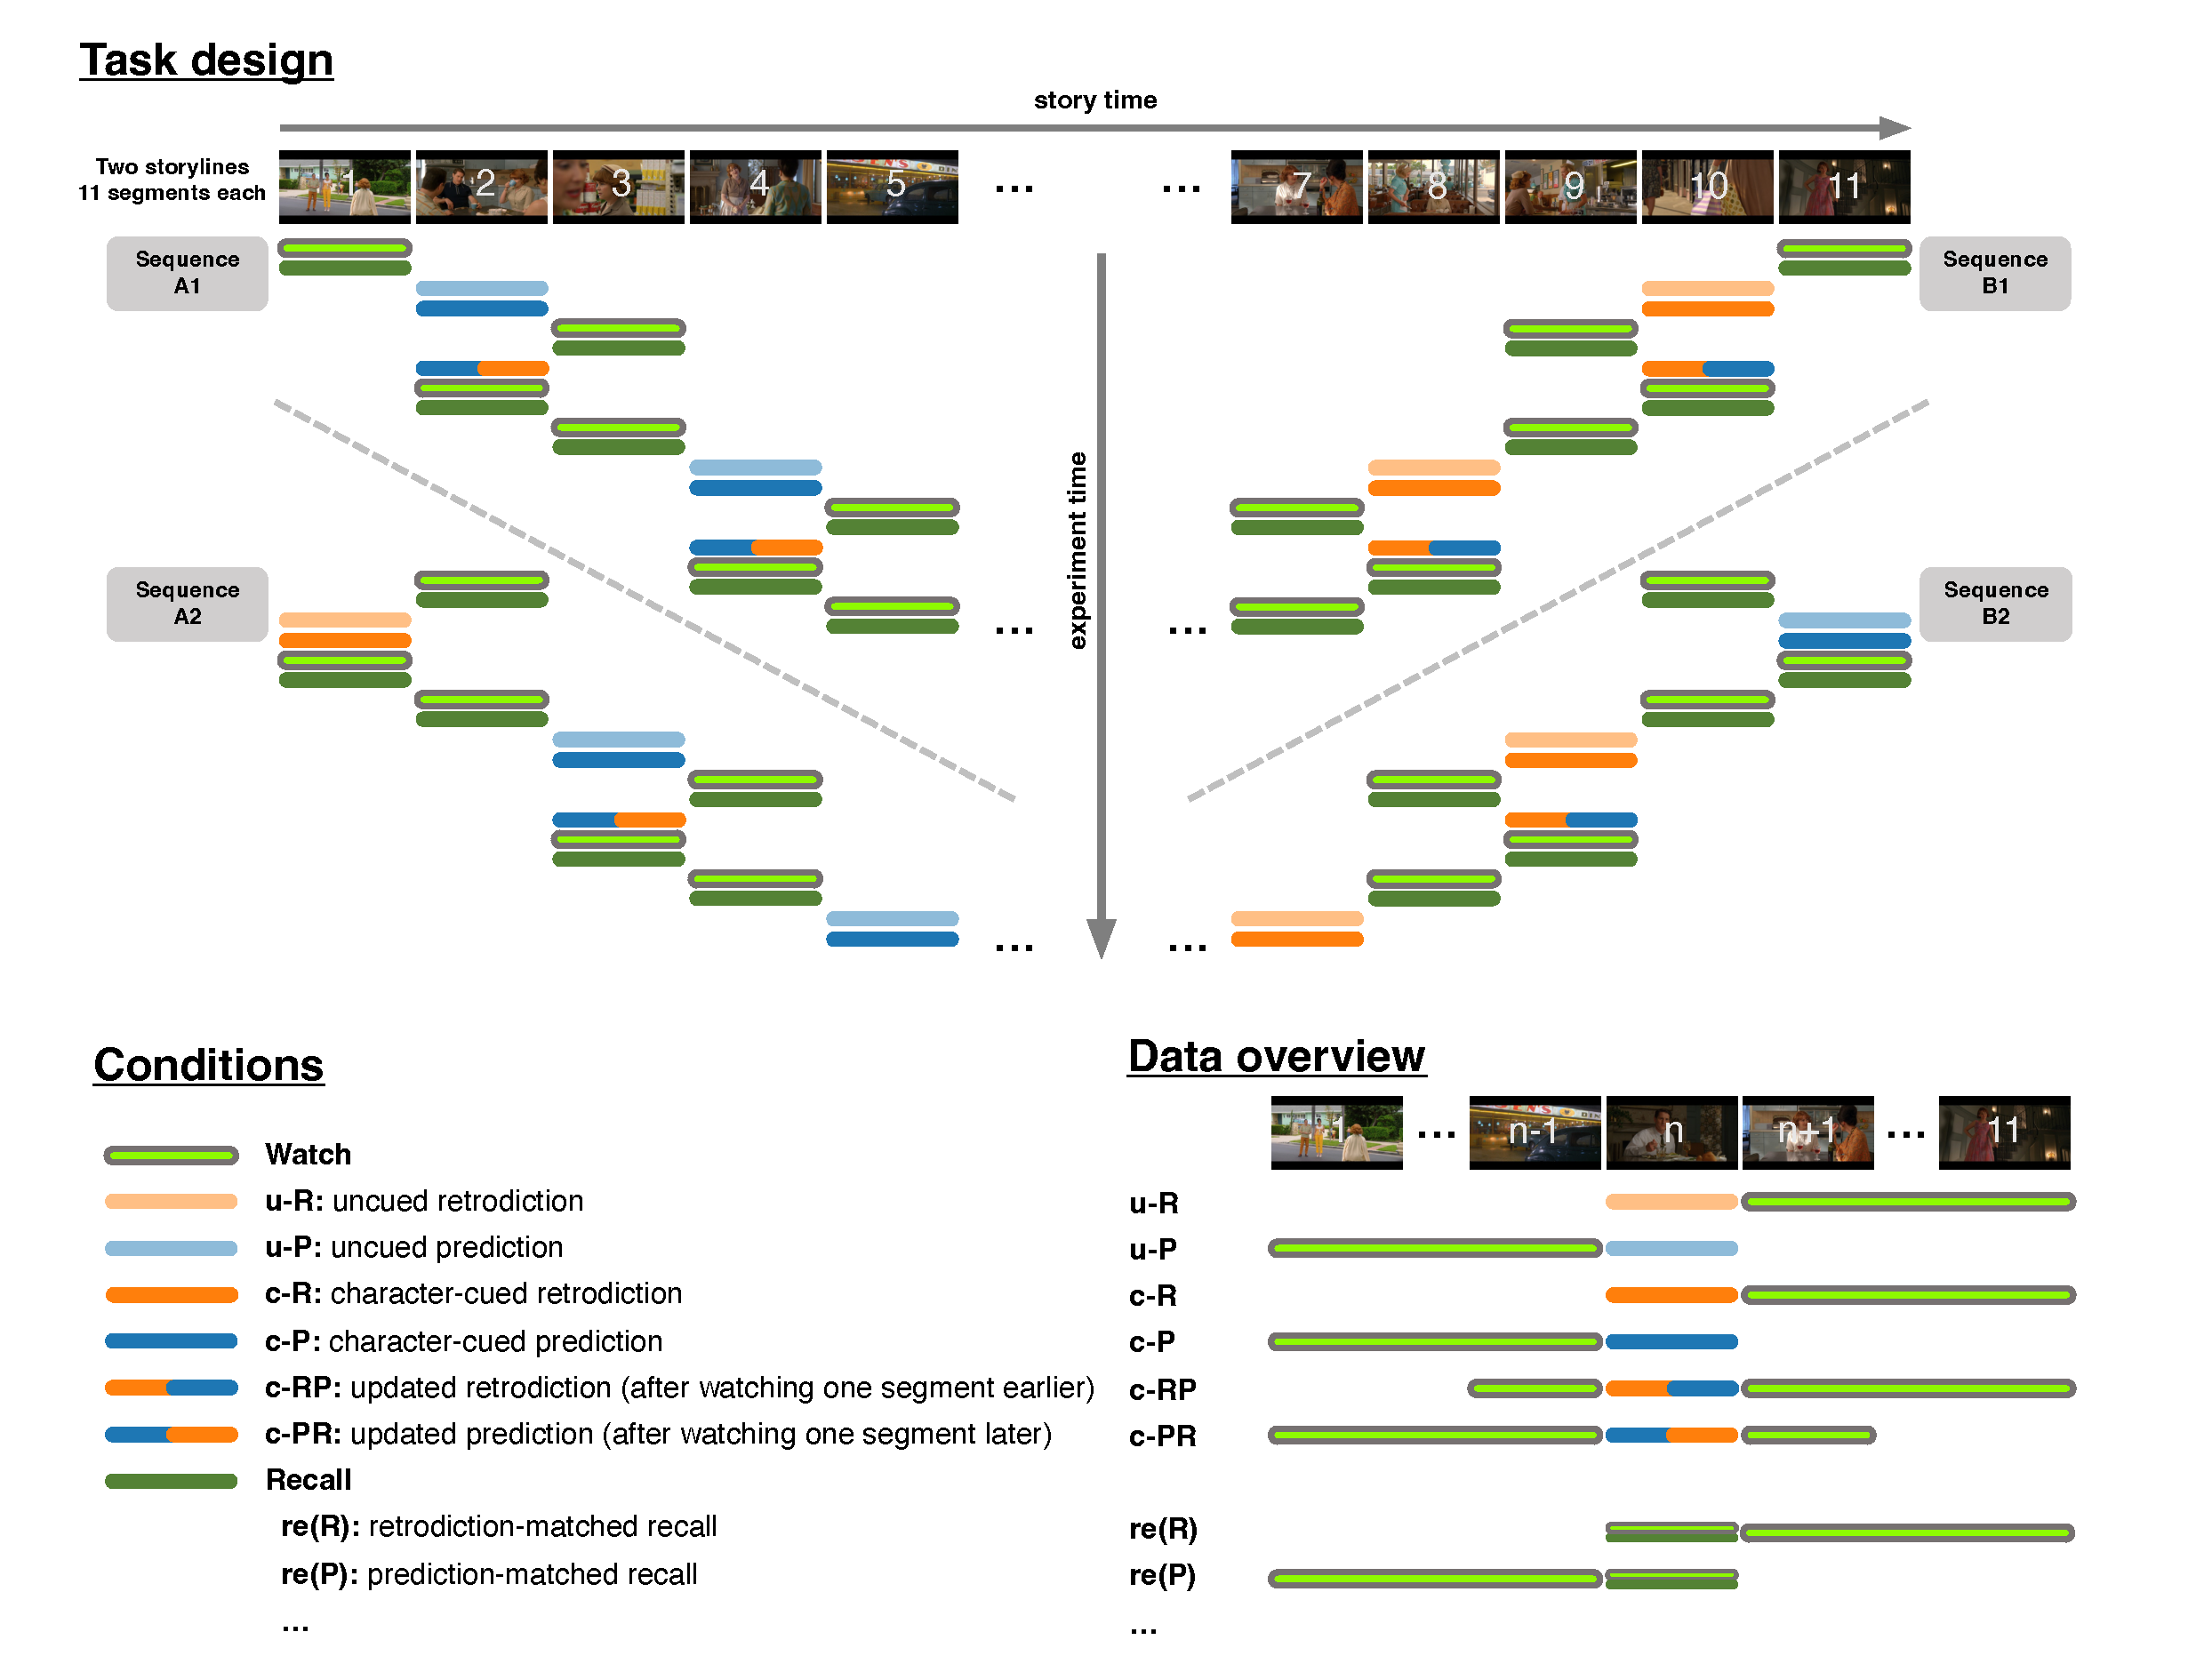
\includegraphics[width=\textwidth]{methods}
  \caption{\textbf{Task overview.} Participants watched segments of two storylines from the television series \textit{Why Women Kill}.  They made free-form text responses to either retrodict what had happened in the previous segment, predict what would happen in the next segment, or recall what happened in the just-watched segment. Across four counterbalanced sequences, we systematically varied whether participants watched the segments in forward or reverse chronological order, whether (or not) responses were cued using the main characters in the target segment, and which other segments participants had watched prior to making a response.  For each segment, we collected several retrodiction, prediction, and/or recall responses across different experimental conditions.}
  \label{fig:method}
\end{figure}


We asked participants to generate four types of responses after watching each video segment: uncued responses, character-cued responses, updated responses, and recalls (Fig.~\ref{fig:method}, \textit{Data overview}).  To generate \textit{uncued} responses, we asked participants to either retrodict (uncued retrodiction; \textit{u-R}) what happened shortly before or predict (uncued prediction; \textit{u-P}) what happened shortly after the just-watched segment.  To generate \textit{character-cued} responses, we asked participants to retrodict (character-cued retrodiction; \textit{c-R}) or predict (character-cued prediction; \textit{c-P}) what came before or after the just-watched segment, but we provided additional information to the participant about which character(s) would be present in the target (to-be-retrodicted or to-be-predicted) segment.  We hypothesized that character-cued responses should be more accurate than uncued responses, to the extent that participants incorporate the character information we provided to them into their retrodictions and predictions.  To generate updated responses, we asked participants to watch an additional segment that came just prior to or just after the target segment, and then to update their retrodiction (\textit{c-RP}) or prediction (\textit{c-PR}) about the target segment. Results on updated responses are not reported in this paper. Finally, we also asked participants to \textit{recall} what happened in the just-watched segment.  We labeled these responses according to which other segments participants had watched prior to the just-watched target.  Retrodiction-matched recall (\textit{re(R)}) responses were made during the retrodiction sequences (B1 and B2; Fig.~\ref{fig:method}), whereas prediction-matched recall (\textit{re(P)}) responses were made during the prediction sequences (A1 and A2).  Participants' recalls provided us with a benchmark for examining information about the participants' experiences and memories, without asking the participants to explicitly speculate about the unobserved.



For each retrodiction and prediction, participants were asked to generate at least one, and not more than three, responses that constituted ``the sorts of things [the participant would] expect to have remembered if [they] had watched the [target] segment.''  They were asked to generate multiple responses only if those additional responses were (in their judgement) of equal likelihood to occur.  On average, participants generated 1.08 responses per prompt; therefore we chose to consider only participants' first (``most probable'' or ``most important'') responses to each prompt.  We also discarded a small number ($n = 20$) of character-cued responses that did not contain references to all cued characters, along with one additional response due to the participant's misunderstanding of the task instructions during that trial.  We carried out our analyses on the remaining 2084 retrodiction, prediction, and recall responses.

\begin{figure}[tp]
  \centering
  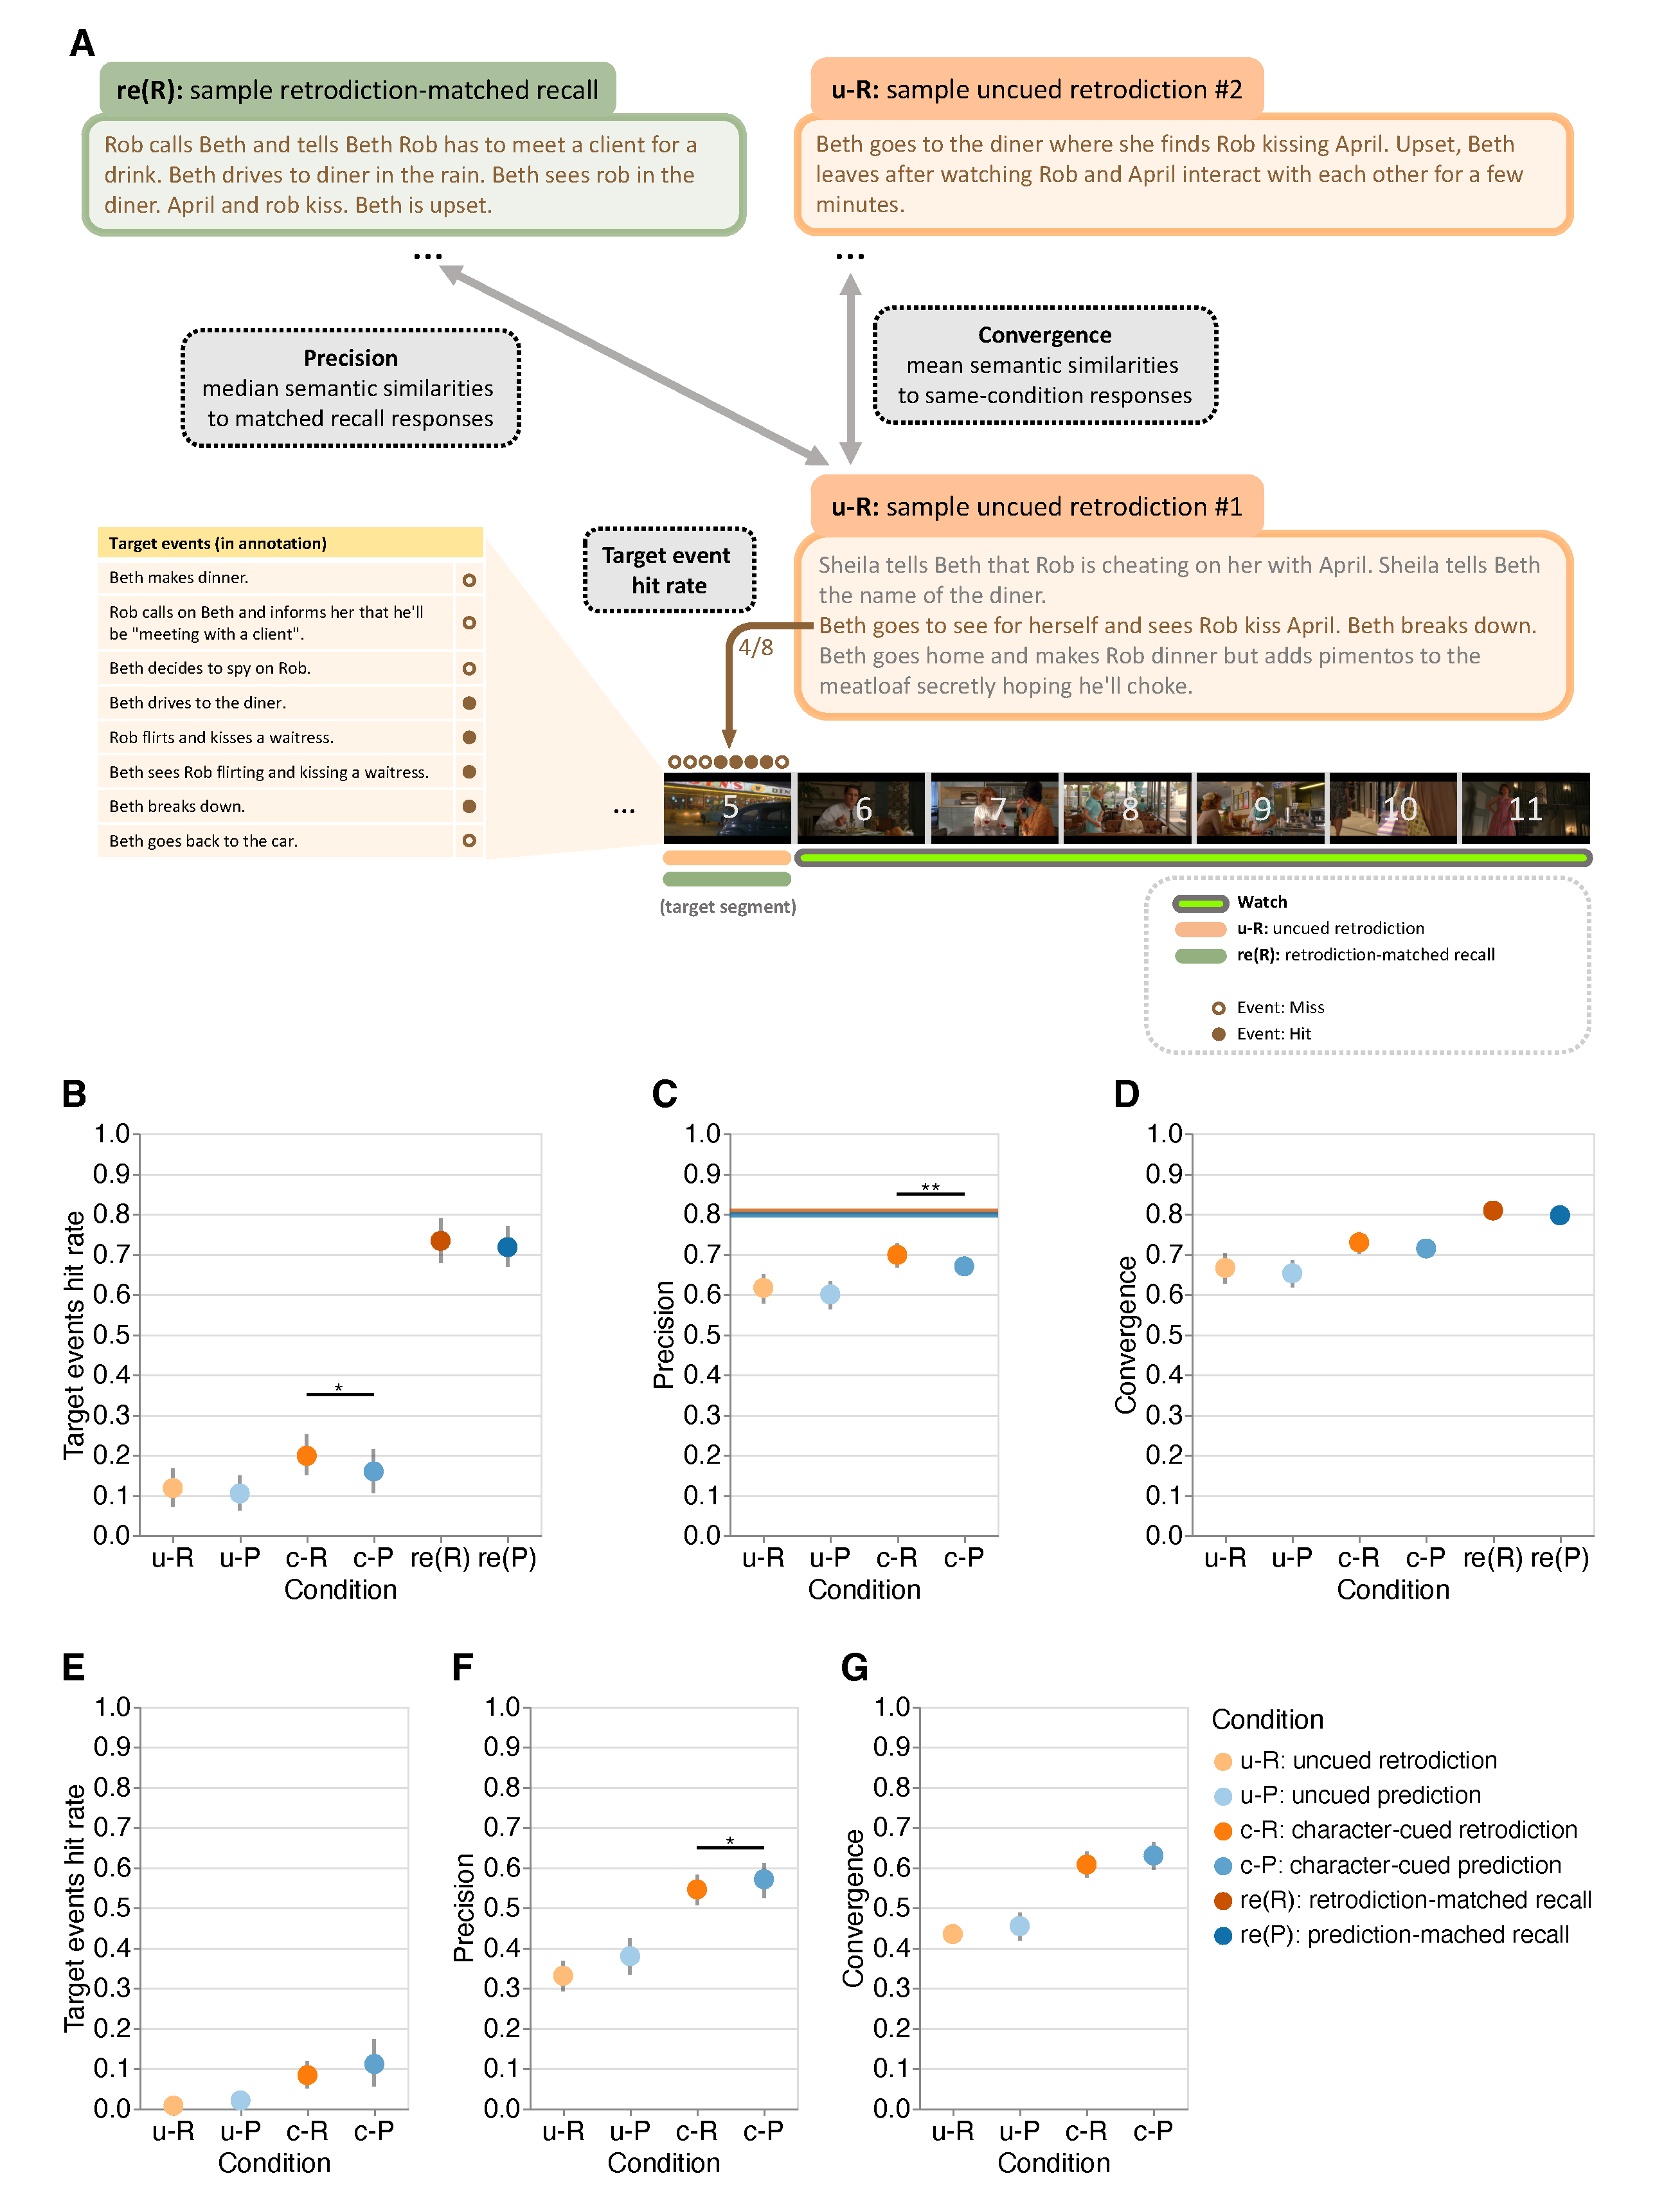
\includegraphics[width=0.80\textwidth]{results1}
  \caption{\textbf{Retrodiction, prediction, and recall performance by experimental condition.} \textbf{A.  Methods schematic.}  For each retrodiction, prediction, and recall response, we calculated the hit rate for events in the target segment, the response precision (see \textit{Methods}), and the response convergence across participants (see \textit{Methods}).  \textbf{B. Target event hit rate.} Mean proportions of target events that were contained in participants' responses, for each response type, averaged across target segments.  \textbf{C. Response precision.}  Mean precisions of participants' responses, for each response type, averaged across target segments.  The horizontal lines denote the mean pairwise semantic similarities (see \textit{Methods}) across recall responses (re(R): orange; re(P): blue).  \textbf{D. Response convergence.}  Mean (across-participant) convergence of participants' responses, for each response type, averaged across target segments.  All panels: error bars denote bootstrapped 95\% confidence intervals.  Asterisks indicate significance in the (generalized) linear mixed models: * denotes $p < 0.05$ and ** denotes $p < 0.01$.}
  \label{fig:result1}
\end{figure}

We used two general approaches to assess the quality of participants' responses (see \textit{Methods}, Fig.~\ref{fig:result1}A).  One approach entailed manually annotating events in the video and counting the number of matched events in participants' responses.  We identified a total of 117 unique events reflected across the 22 video segments (range: 3--9 per segment; see \textit{Methods}, Table \stimDescription).  We assigned one ``point'' to each of these video events.  We also identified 23 additional events in participants' responses that were either summaries of several events or that were partial matches to the manually identified video events.  We assigned 0.5 point to each of these additional events.  This point system enabled us to compute the numbers and proportions (\textit{hit rates}) of correctly retrodicted, predicted, and recalled events contained in each response.  Our second approach entailed using a natural language processing model~\citep{CerEtal18} to embed annotations and responses in a 512-dimensional feature space.  This approach was designed to capture conceptual overlap between responses that were not necessarily tied to specific events.  To quantify this conceptual overlap, we computed the similarities between the embeddings of different sets of responses.  Following \cite{HeusEtal21}, we defined the \textit{precision} of each participants' retrodictions or predictions about a given segment as the median cosine similarities between the embeddings of (a) the participant's retrodiction or prediction response for the given segment and (b) each \textit{other} participant's recalls of the same segment.  In other words, precision is designed to measure the extent to which retrodictions and predictions captured the conceptual content that (other) participants remembered.  We also developed a related measure, which we call \textit{convergence}, to characterize response similarities across participants.  In particular, we defined convergence as the mean cosine similarity between the embeddings of a participant's responses to a given target segment and all other participants' responses (of the same type) to the same segment.  We analyzed the data using generalized linear mixed models, with participant and stimulus (e.g., target segment) identities as crossed random effects (see \textit{Methods}).

First we sought to validate a main effect of response type (i.e., uncued responses, character-cued responses, and recalls), irrespective of the temporal direction (retrodiction versus prediction).  Across these three types of responses, participants have access to increasing amounts of information about the target segment.  Therefore, across these response types, we hypothesized that participants' responses should become both more accurate and more convergent across individuals.  Consistent with this hypothesis, participants' character-cued retrodictions and predictions were associated with higher target event hit rates than uncued retrodictions and predictions (odds ratio (OR): 2.65, $Z = 4.24$, $p < 0.001$, 95\% confidence interval (CI): 1.69 to 4.16; Fig.~\ref{fig:result1}B).  These character-cued responses were also more precise ($b = 0.13$, $t(18.1) = 9.43$, $p < 0.001$, CI: 0.10 to 0.16; Fig.~\ref{fig:result1}C) and convergent across individuals ($b = 0.11$, $t(18.6) = 6.21$, $p < 0.001$, CI: 0.07 to 0.15; Fig.~\ref{fig:result1}D).   Relative to character-cued responses, participants' recalls showed higher target event hit rates (OR = 21.83, $Z = 10.61$, $p < 0.001$, CI: 12.35 to 38.59) and more convergence across individuals ($b = 0.20$, $t(19.4) = 9.10$, $p < 0.001$, CI: 0.16 to 0.25). These results are consistent with the common-sense notion that access to more information about a target segment yields better performance (i.e., higher hit rates, precision, and convergence across individuals).

Next we carried out a series of analyses specifically aimed at characterizing temporal direction effects--- i.e, the relative quality of retrodictions versus predictions across different types of responses.  We hoped that these analyses might provide insights into our central question about whether the present is equally informative about the past and future.  Across both uncued and character-cued responses (Fig.~\ref{fig:method}), retrodictions had numerically higher hit rates than predictions (Fig.~\ref{fig:result1}B).  However, these differences were only statistically reliable for character-cued responses (uncued responses: OR = 1.17, $Z = 0.35$, $p = 0.73$, CI: 0.47 to 2.92; character-cued responses: OR = 1.93, $Z = 2.15$, $p = 0.03$, CI: 1.06 to 3.52).  We observed a similar pattern of results for the precisions of participants' responses (Fig.~\ref{fig:result1}C).  Specifically, their responses tended to be numerically more precise for retrodictions versus predictions, but the differences were only statistically reliable for character-cued responses (uncued responses: $b = 0.03$, $t(20.9) = 1.09$, $p = 0.29$, CI: -0.03 to 0.10; character-cued responses: $b = 0.06$, $t(20.8) = 3.01$, $p = 0.007$, CI: 0.02 to 0.11).  We also consistently observed numerically higher convergence across participants for retrodictions versus predictions (Fig.~\ref{fig:result1}D), but neither of these differences were statistically reliable (uncued responses: $b = 0.03$, $t(17.9) = 0.75$, $p = 0.46$, CI: -0.05 to 0.11; character-cued responses: $b = 0.04$, $t(17.4) = 1.46$, $p = 0.16$, CI: -0.02 to 0.09).  Because the retrodiction versus prediction performance differences we observed were only statistically reliable when participants were cued with the target segments' characters, this suggests that information about the unobserved past versus the unobserved future may differently affect retrodictions versus predictions.  Taken together, these results suggest that participants are generally better at making retrodictions than predictions.  We also verified that this was not solely a consequence of how participants' memory performance might have been affected by watching different segments (or making different responses to other segments) across conditions by comparing recall responses in the retrodiction-matched recall (\textit{re(R)}) and prediction-matched recall (\textit{re(P)}) conditions.  Recall performance was similar in both conditions (target event hit rate: OR = 1.12, $Z = 1.07$, $p = 0.29$, CI: 0.91 to 1.39; convergence: $b = 0.03$, $t(19.3) = 1.89$, $p = 0.07$, CI: 0.00 to 0.07).

\begin{figure}[tp]
  \centering
  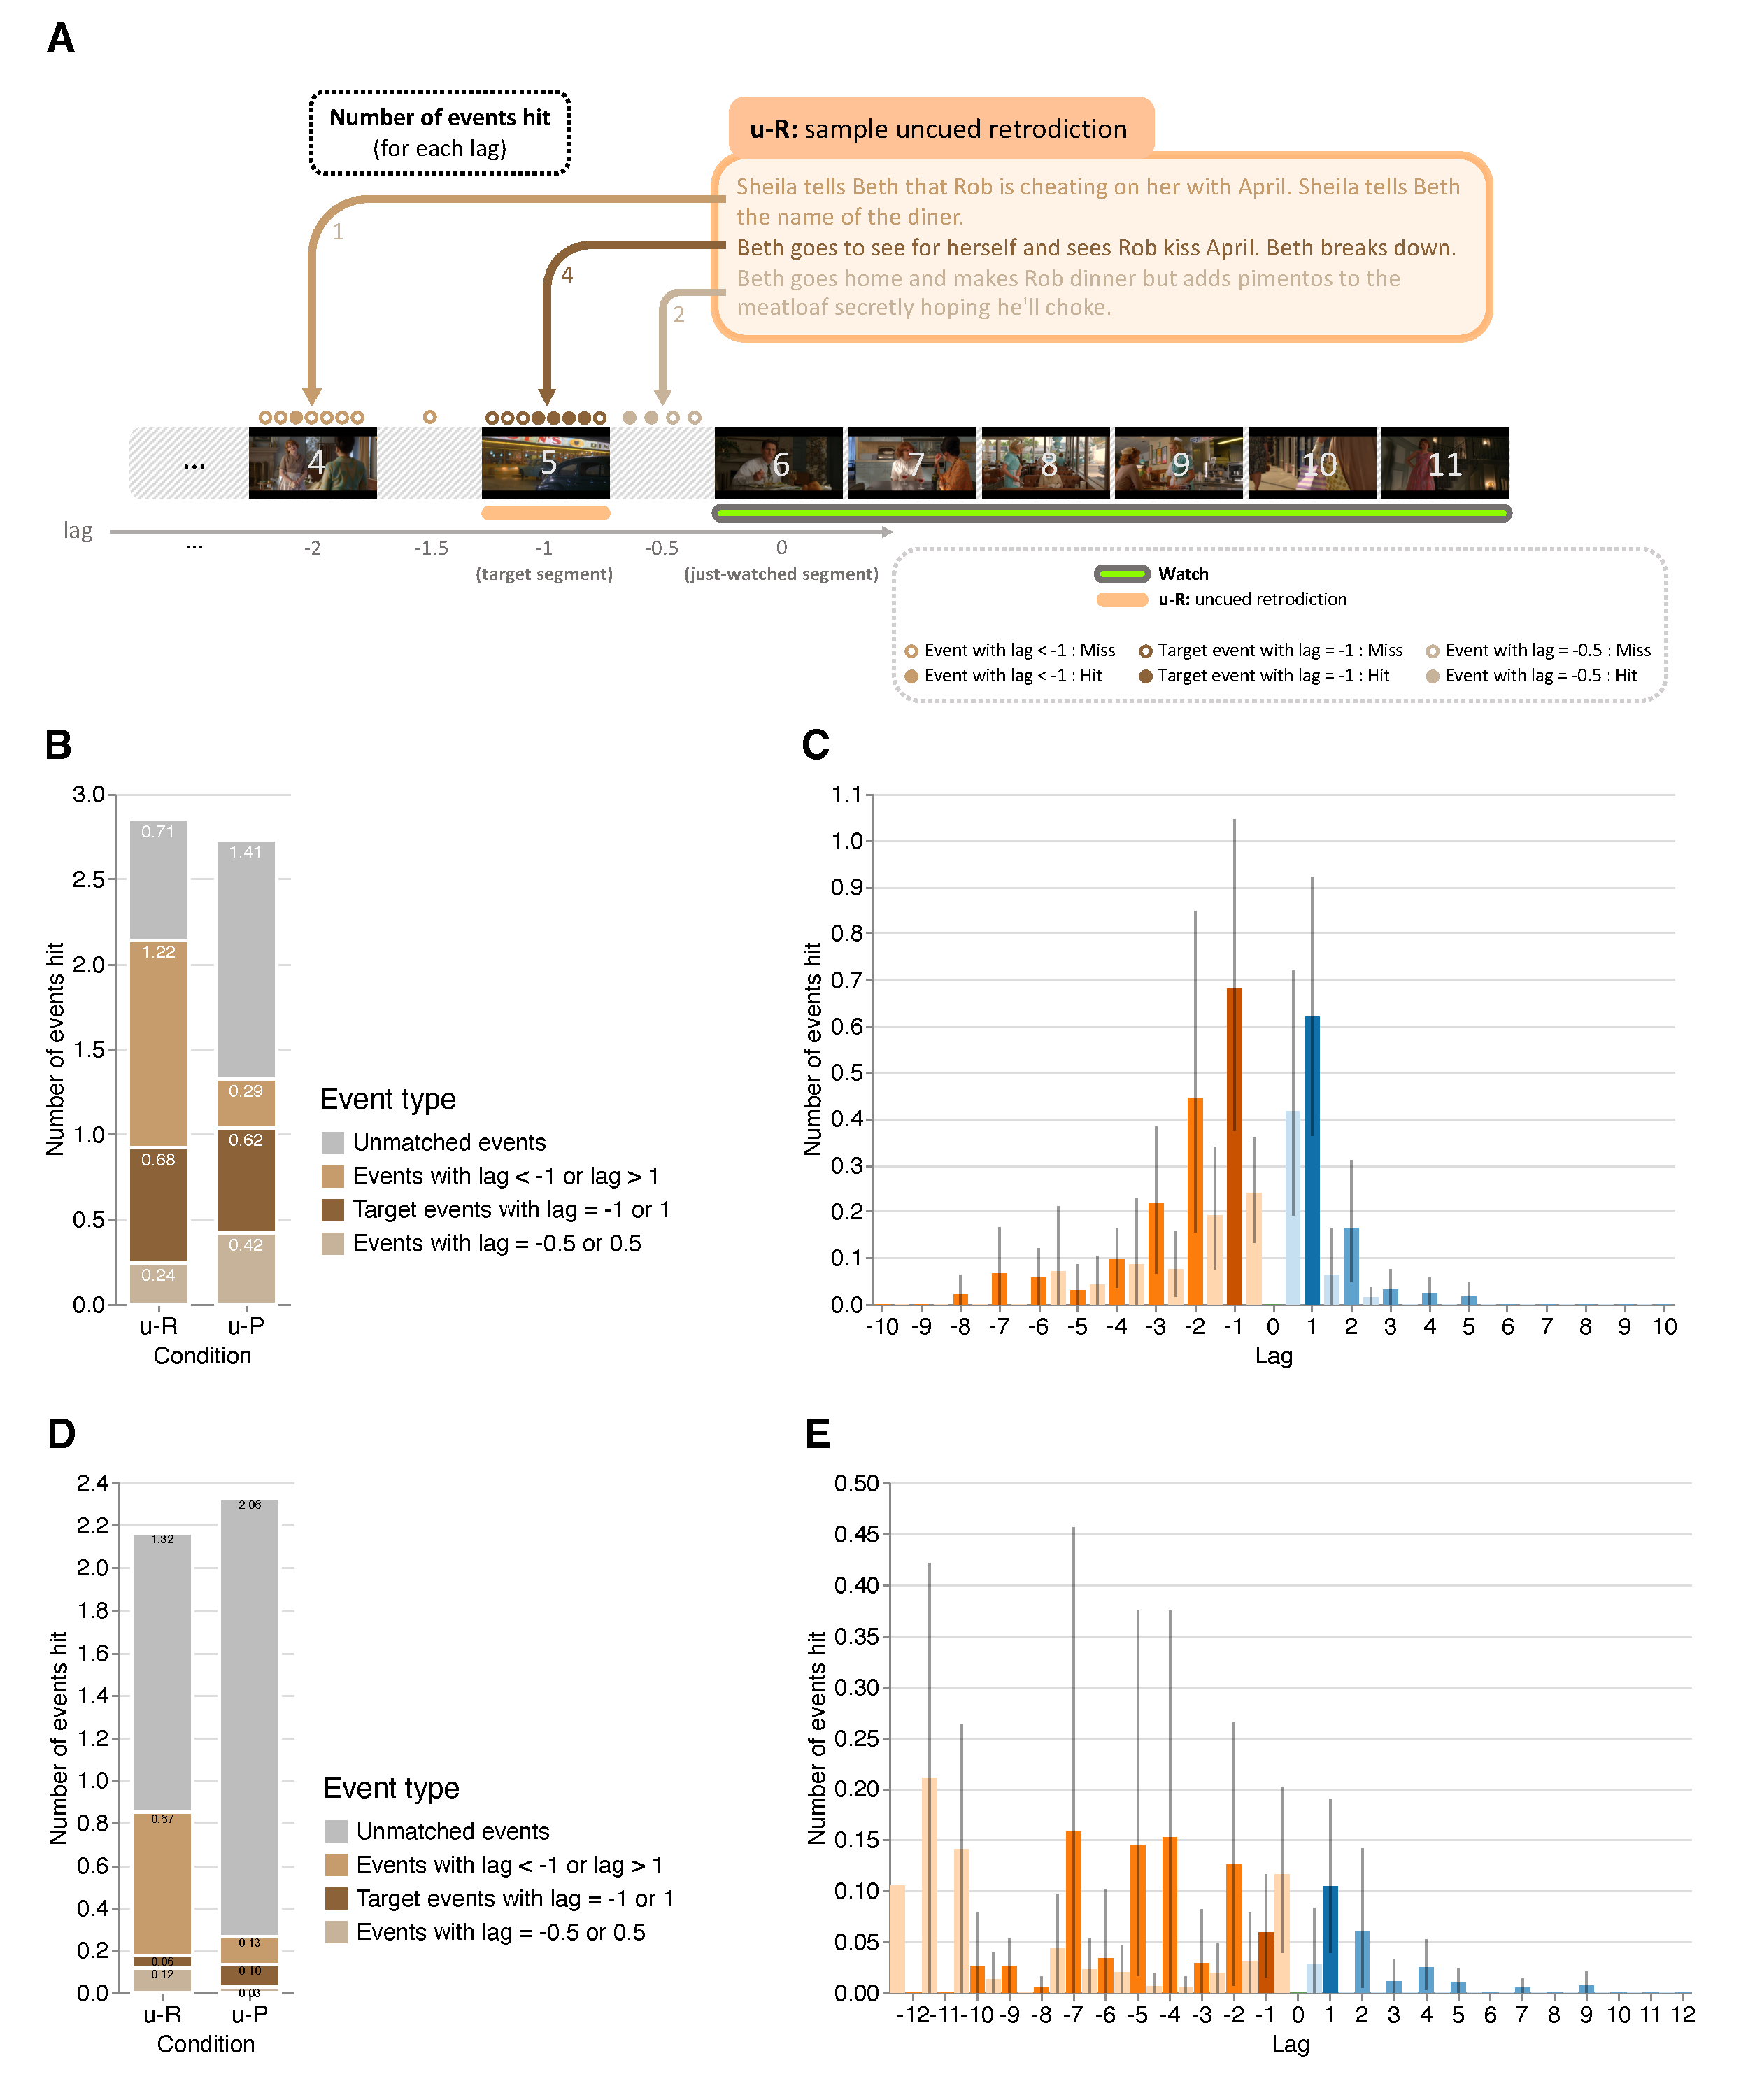
\includegraphics[width=\textwidth]{results2}
  \caption{\textbf{Retrodictions and predictions of temporally near and distant events.}  \textbf{A. Illustration of annotation approach.}  For each uncued retrodiction and prediction response, we calculated the number of (retrodicted or predicted) events as a function of temporal distance from the target segment, or \textit{lag}.  Onscreen (explicit) events are tagged using integer-valued lags, whereas offscreen (implicit) events are tagged using half-step lags ($\pm 0.5$, $\pm 1.5$, etc.).  \textbf{B. Number of events hit in participants' uncued retrodictions and predictions for each event type.}  Here we separated events we identified in participants' responses according to whether they occurred in the target segment (lags of $\pm 1$), during the interval between the target segment and the just-watched segment (lags of $\pm 0.5$), at longer temporal distances ($|\mathrm{lag}| > 1$), or were incorrect (unmatched with any past or future events in the narrative).  The counts displayed in the panel are averaged across just-watched segments.  \textbf{C. Number of events hit as a function of temporal distance.}  Here the (across-segment) mean numbers of events hit in participants' uncued retrodictions (orange) and predictions (blue) are displayed as a function of temporal distance to the just-watched segment (lag).  Error bars denote bootstrapped 95\% confidence intervals.  Colors denote temporal direction (orange: past; blue: future) and distance (darker shading: onscreen events from segments adjacent to the target segment; lighter shading: offscreen events).}
  \label{fig:result2}
\end{figure}

The above analyses were focused solely on the target segment (i.e., retrodiction of segment $i - 1$ after watching segments $i...11$, or prediction of segment $i + 1$ after watching segments $1...i$).  We wondered whether participants' responses might also contain longer-range information about preceding or proceeding events.  In order to carry out this analysis properly, we reasoned that participants might reference past or future events that were \textit{implied} to have occurred offscreen, but not explicitly shown onscreen.  For example, a character in location A during one scene might appear in location B during the immediately following scene.  Although it wasn't shown onscreen, we can infer that the character traveled between locations A and B sometime between the time intervals separating the scenes~\citep{Bord08}.  In all, we manually identified a set of 74 \textit{implicit} offscreen events that were implied to have occurred given what was (explicitly) depicted onscreen (Fig.~\ref{fig:result2}A), plus one additional partial event and one additional summary event.  We defined the just-watched segment as having a \textit{lag} of 0.  We assigned the target segment of a participant's retrodiction or prediction (i.e., the immediately preceding or proceeding segment) a lag of -1 or +1, respectively.  The segment following the next was assigned a lag of 2, and so on.  We tagged offscreen events using half steps.  For example, an offscreen event that occurred after the prior segment but before the just-watched segment would be assigned a lag of -0.5.

Because there is no ``ground truth'' number of offscreen events, we could not compute the hit rates for offscreen events.  Instead, we counted up the absolute \textit{number} of retrodicted or predicted events as a function of lag.  In other words, given that the participant had just watched segment $i$, we asked how many events from segment $i + lag$ they retrodicted or predicted, on average, given that they were aiming to retrodict or predict events at lags of $\pm 1$.  We also counted the numbers of \textit{unmatched} events in participants' responses that did not correspond to any events in the relevant segments of the narrative.  We focused specifically on \textit{uncued} retrodictions and predictions, which we hypothesized would provide the cleanest characterizations of participants' initial estimates of the unobserved past and future (i.e., without potential biases introduced by additional character information, as in the character-cued responses).  The numbers of uncued retrodicted and predicted target (lag = $\pm 1$) events were not reliably different (OR = 0.92, $Z = -0.15$, $p = 0.88$, CI: 0.30 to 2.84).  In other words, uncued retrodictions and predictions over short timescales did not exhibit reliable asymmetries.  However, when retrodicting, participants mentioned events from the distant past ($\mathrm{lag} < -1$) more often than participants predicted events from the distant future ($\mathrm{lag} > 1$; OR = 9.10, $Z = 3.80$, $p < 0.001$, CI: 2.92 to 28.39; Fig.~\ref{fig:result2}B, C; for results from the character-cued conditions, see Fig.~\events).  Despite this asymmetry in the accuracies of participants' long-range retrodictions versus predictions, there were no reliable differences in the \textit{numbers} of uncued retrodicted versus predicted events (across all lags; OR = 1.05, $Z = 0.75$, $p = 0.45$, CI: 0.93 to 1.18).  Nor did we find any reliable differences in the numbers of offscreen events immediately before or after the just-watched segment ($lag = \pm 0.5$; OR = 0.75, $Z = -0.36$, $p = 0.72$, CI: 0.15 to 3.59).  The apparent discrepancy between participants' asymmetric accuracy but symmetric event counts was due to participants' tendencies to reference ``unmatched'' events (i.e., events that did not correspond to any explicit or implicit event in the story) more in their predictions than retrodictions (OR = 0.36, $Z = -4.53$, $p < 0.001$, CI: 0.23 to 0.56).  We confirmed that the retrodiction advantage held when controlling for absolute lag (OR = 34.31, $Z = 3.28$, $p = 0.001$, CI: 4.16 to 283.20), for onscreen events alone (OR = 47.54, $Z = 3.74$, $p < 0.001$, CI: 6.27 to 360.60), and marginally for offscreen events alone (OR = 24.76, $Z = 1.71$, $p = 0.09$, CI: 0.63 to 975.27).  Taken together, these analyses show that (in generating uncued responses) participants tend to reach ``further'' into the unobserved past, and with greater accuracy, than the unobserved future.

\begin{figure}[tp]
  \centering
  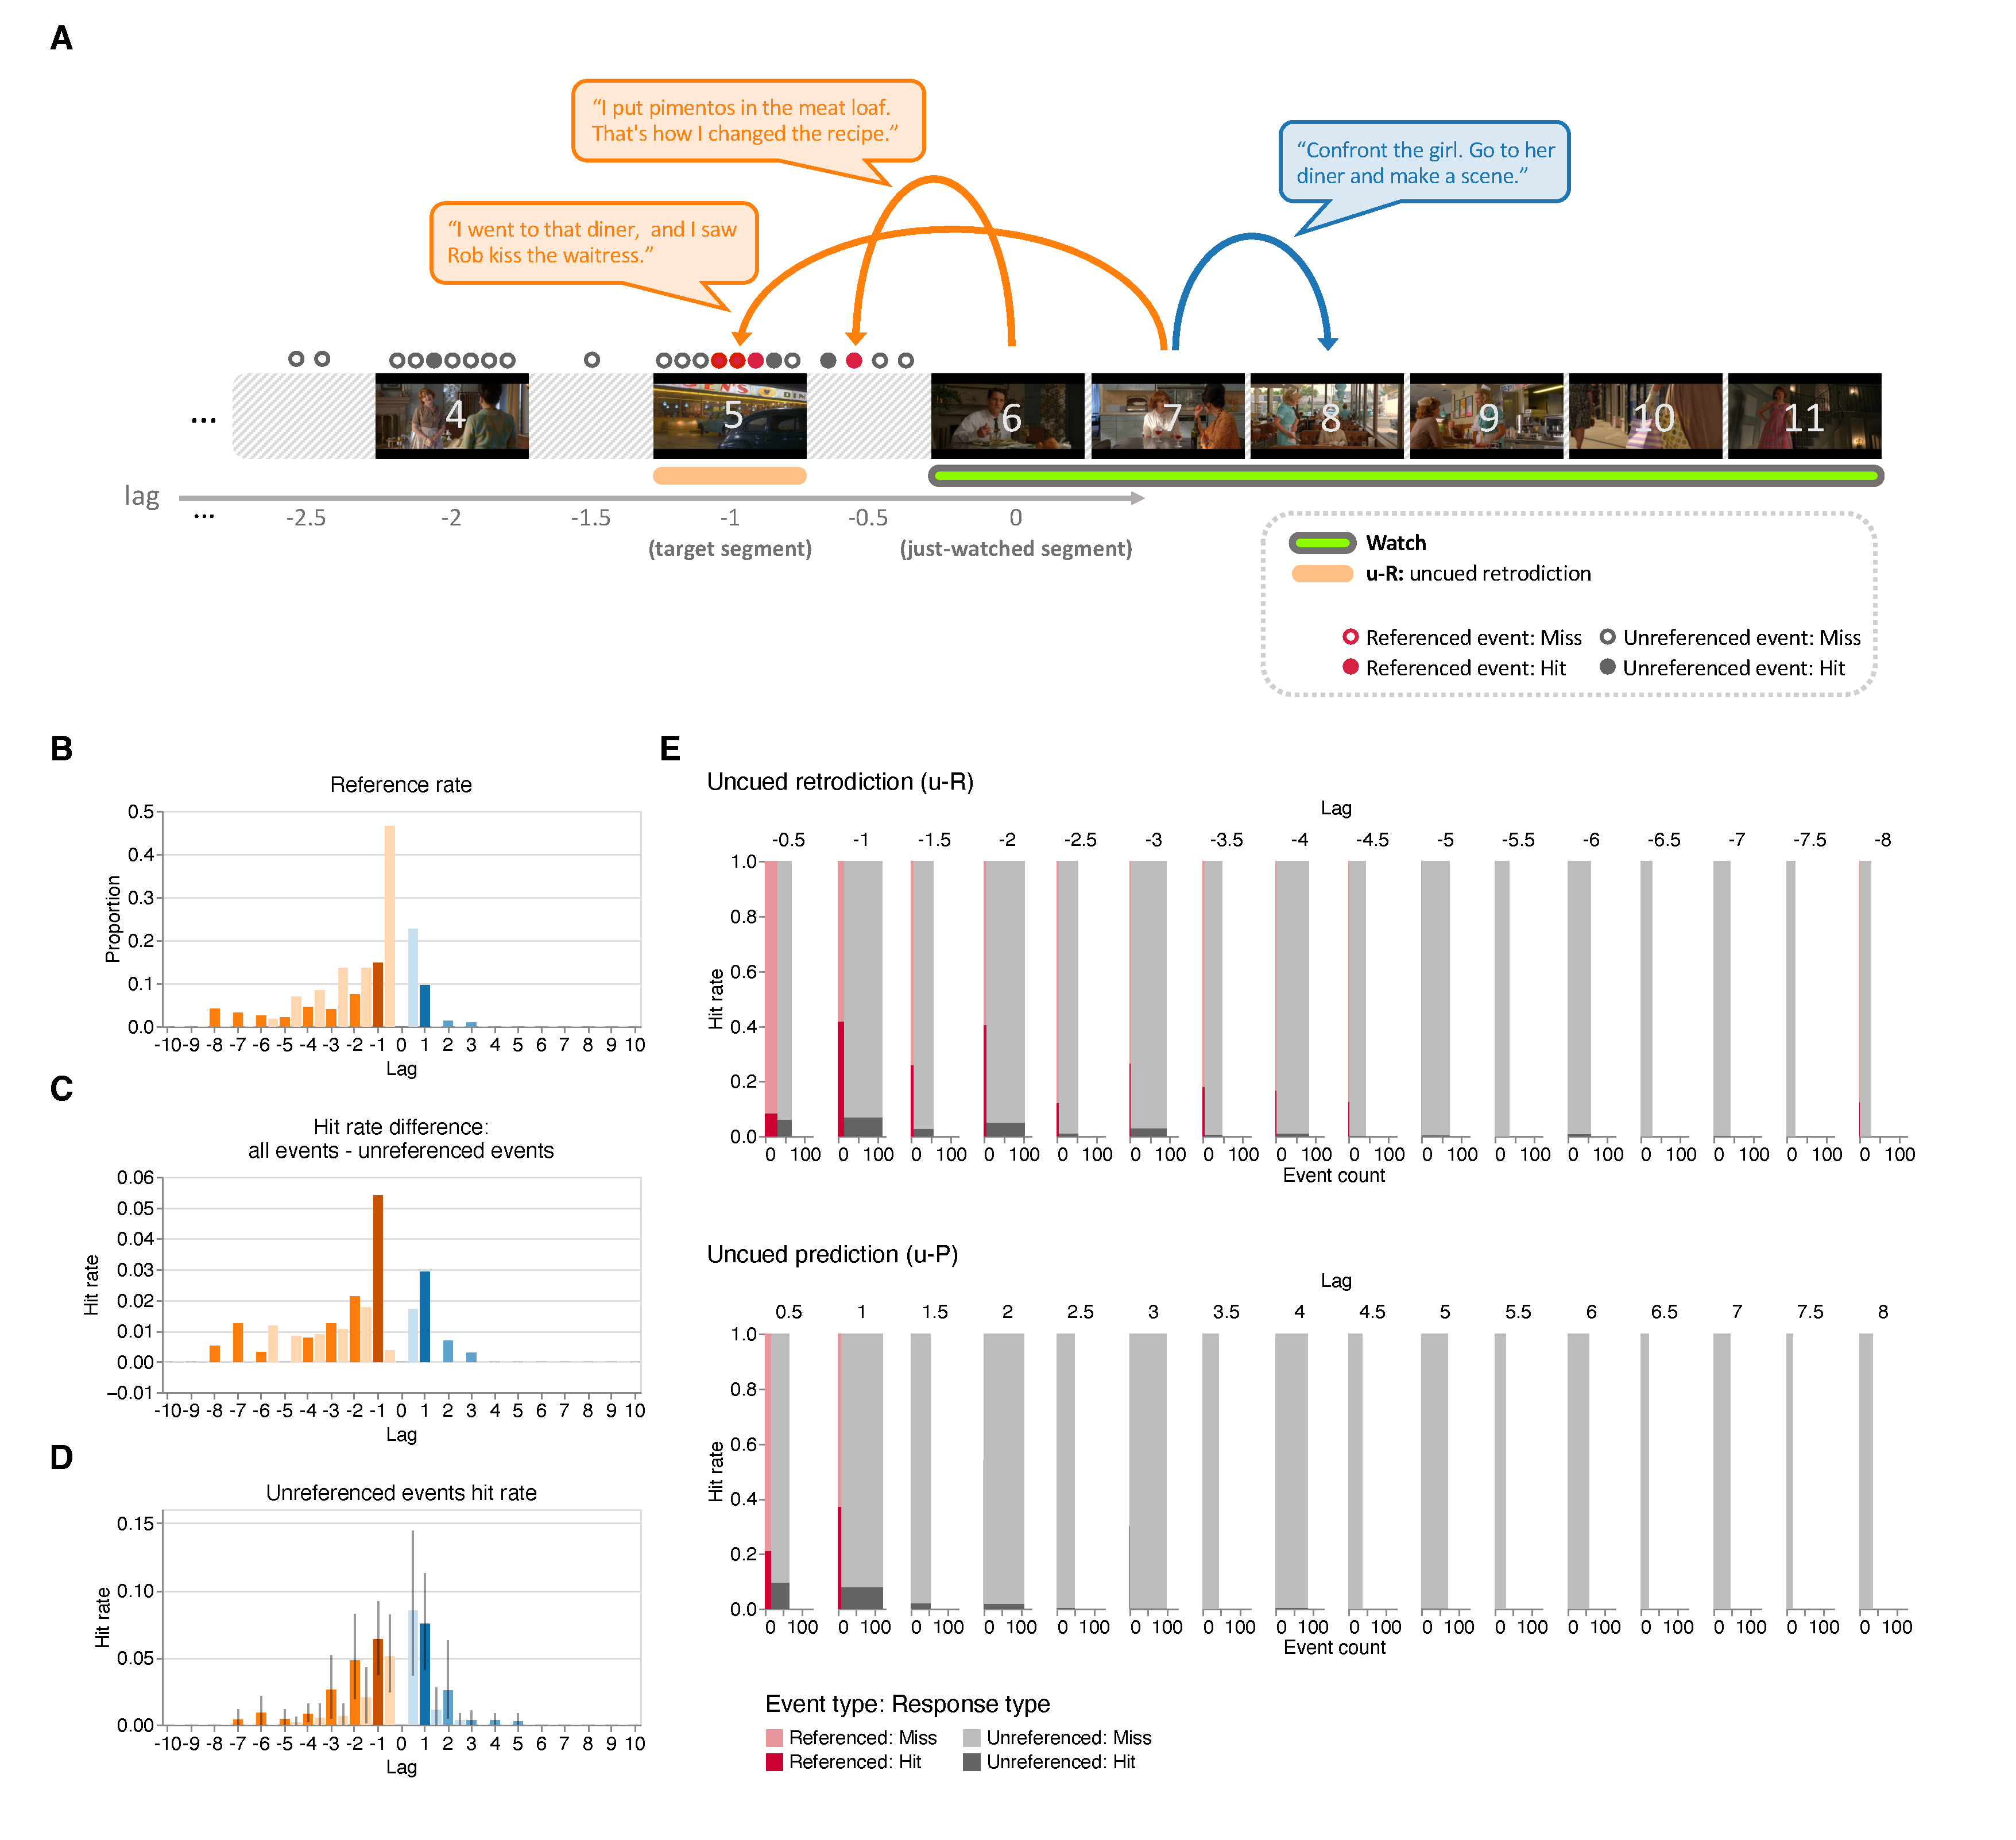
\includegraphics[width=0.9\textwidth]{results3}
  \caption{\textbf{Characters' references drive participants' retrodiction and prediction performance.}  \textbf{A. Illustration of annotation approach.}  We manually annotated references to events in past or future segments in characters' spoken conversations.  We matched each such reference with its corresponding storyline event (and its corresponding segment number for onscreen events, or half-step segment number for offscreen events).  We then tracked the hit rate separately for referenced versus unreferenced events, in participants' uncued retrodictions and predictions.  \textbf{B. Reference rate as a function of lag.}  Across all possible just-watched segments (lag 0), the bar heights denote the average proportions of events referenced in other past (orange, negative lags) or future (blue, positive lags) segments.  \textbf{C. Difference in hit rates between all events and unreferenced events.}  To highlight the effect of characters' references to past and future events on participants' retrodictions and predictions, here we display the difference in across-segment mean hit rates between all events and unreferenced events, as a function of temporal distance (lag) to the just-watched segment.  \textbf{D. Hit rates for unreferenced events.}  The average response hit rates for unreferenced events are displayed as a function of temporal distance to the just-watched segment.  Error bars denote bootstrapped 95\% confidence intervals.  Panels B--D: colors are described in the Figure~\ref{fig:result2} caption.  \textbf{E.  Hit rates and counts of referenced and unreferenced events.}  As a function of temporal distance to the just-watched segment, the sub-panels display the across-segment mean numbers ($x$-axes) and hit rates ($y$-axes) of referenced (red) and unreferenced (gray) events that participants hit (darker shading) or missed (lighter shading) in their uncued retrodictions (top sub-panel) and uncued predictions (bottom sub-panel).}
  \label{fig:result3}
\end{figure}

What might be driving participants to retrodict further and more accurately into the unobserved past, compared with their predictions of the unobserved future?  By inspecting the video content, we noticed that characters in the television show frequently referenced both past events and (planned or predicted) future events in their spoken conversations.  We wondered whether the characters' references might show temporal asymmetries that might explain participants' behaviors.  Across all of the characters' conversations, and across all of the video segments, we manually identified a total of 82 references to past or future events (i.e., that occurred onscreen or offscreen before or after the events depicted in the current segment; Fig.~\ref{fig:result3}A, \references A).  Characters tended to reference the past (52 references) more than the future (30 references), consistent with previous work~\citep{DemiEtal18}.  References to the past were also skewed to more temporally distant events compared with references to the future (Figs.~\ref{fig:result3}B,~\references B).  These observations indicate that the characters in the stimulus display a preference for the past (versus future) in their conversations.  Might this asymmetry be driving the asymmetries in participants' retrodictions versus predictions?

Controlling for temporal distance (lag), past and future events that story characters referenced in their conversations were associated with higher hit rates than unreferenced events (uncued retrodiction: OR = 12.70, $Z = 10.94$, $p < 0.001$, CI: 8.06 to 20.03; uncued prediction: OR = 8.29, $Z = 6.83$, $p < 0.001$, CI: 4.52 to 15.20; Fig.~\ref{fig:result3}E).  This indicates that participants' responses are at least partially influenced by the characters' conversations.  
To estimate the contributions of characters’ references on hit rates, we computed the difference in hit rates between all events (which comprised both referenced and unreferenced events) and unreferenced events, as a function of lag. 
These differences exhibited a temporal asymmetry in favor of retrodiction (Fig.~\ref{fig:result3}C).  
This indicates that the asymmetries in participants' retrodictions versus predictions are also at least partially influenced by the characters' conversations. 
However, these temporal asymmetries in participants' retrodictions and predictions persisted even for events that characters never referenced in their conversations (hit rates of uncued retrodicted versus predicted unreferenced events: OR = 2.00, $Z = 2.40$, $p = 0.02$, CI: 1.14 to 3.51; Fig.~\ref{fig:result3}D).  When we further separated the unreferenced events into onscreen events and offscreen events, we found that these asymmetries held only for the onscreen events (onscreen: OR = 2.65, $Z = 2.59$, $p = 0.01$, CI: 1.27 to 5.54; offscreen: OR = 1.50, $Z = 0.91$, $p = 0.36$, CI: 0.63 to 3.62).  Taken together, these analyses suggest that asymmetries in the number of references characters make to past and future events partially (but not entirely) explain why participants tend to retrodict the past further and more accurately than they predict the future.

\begin{figure}[tp]
  \centering
  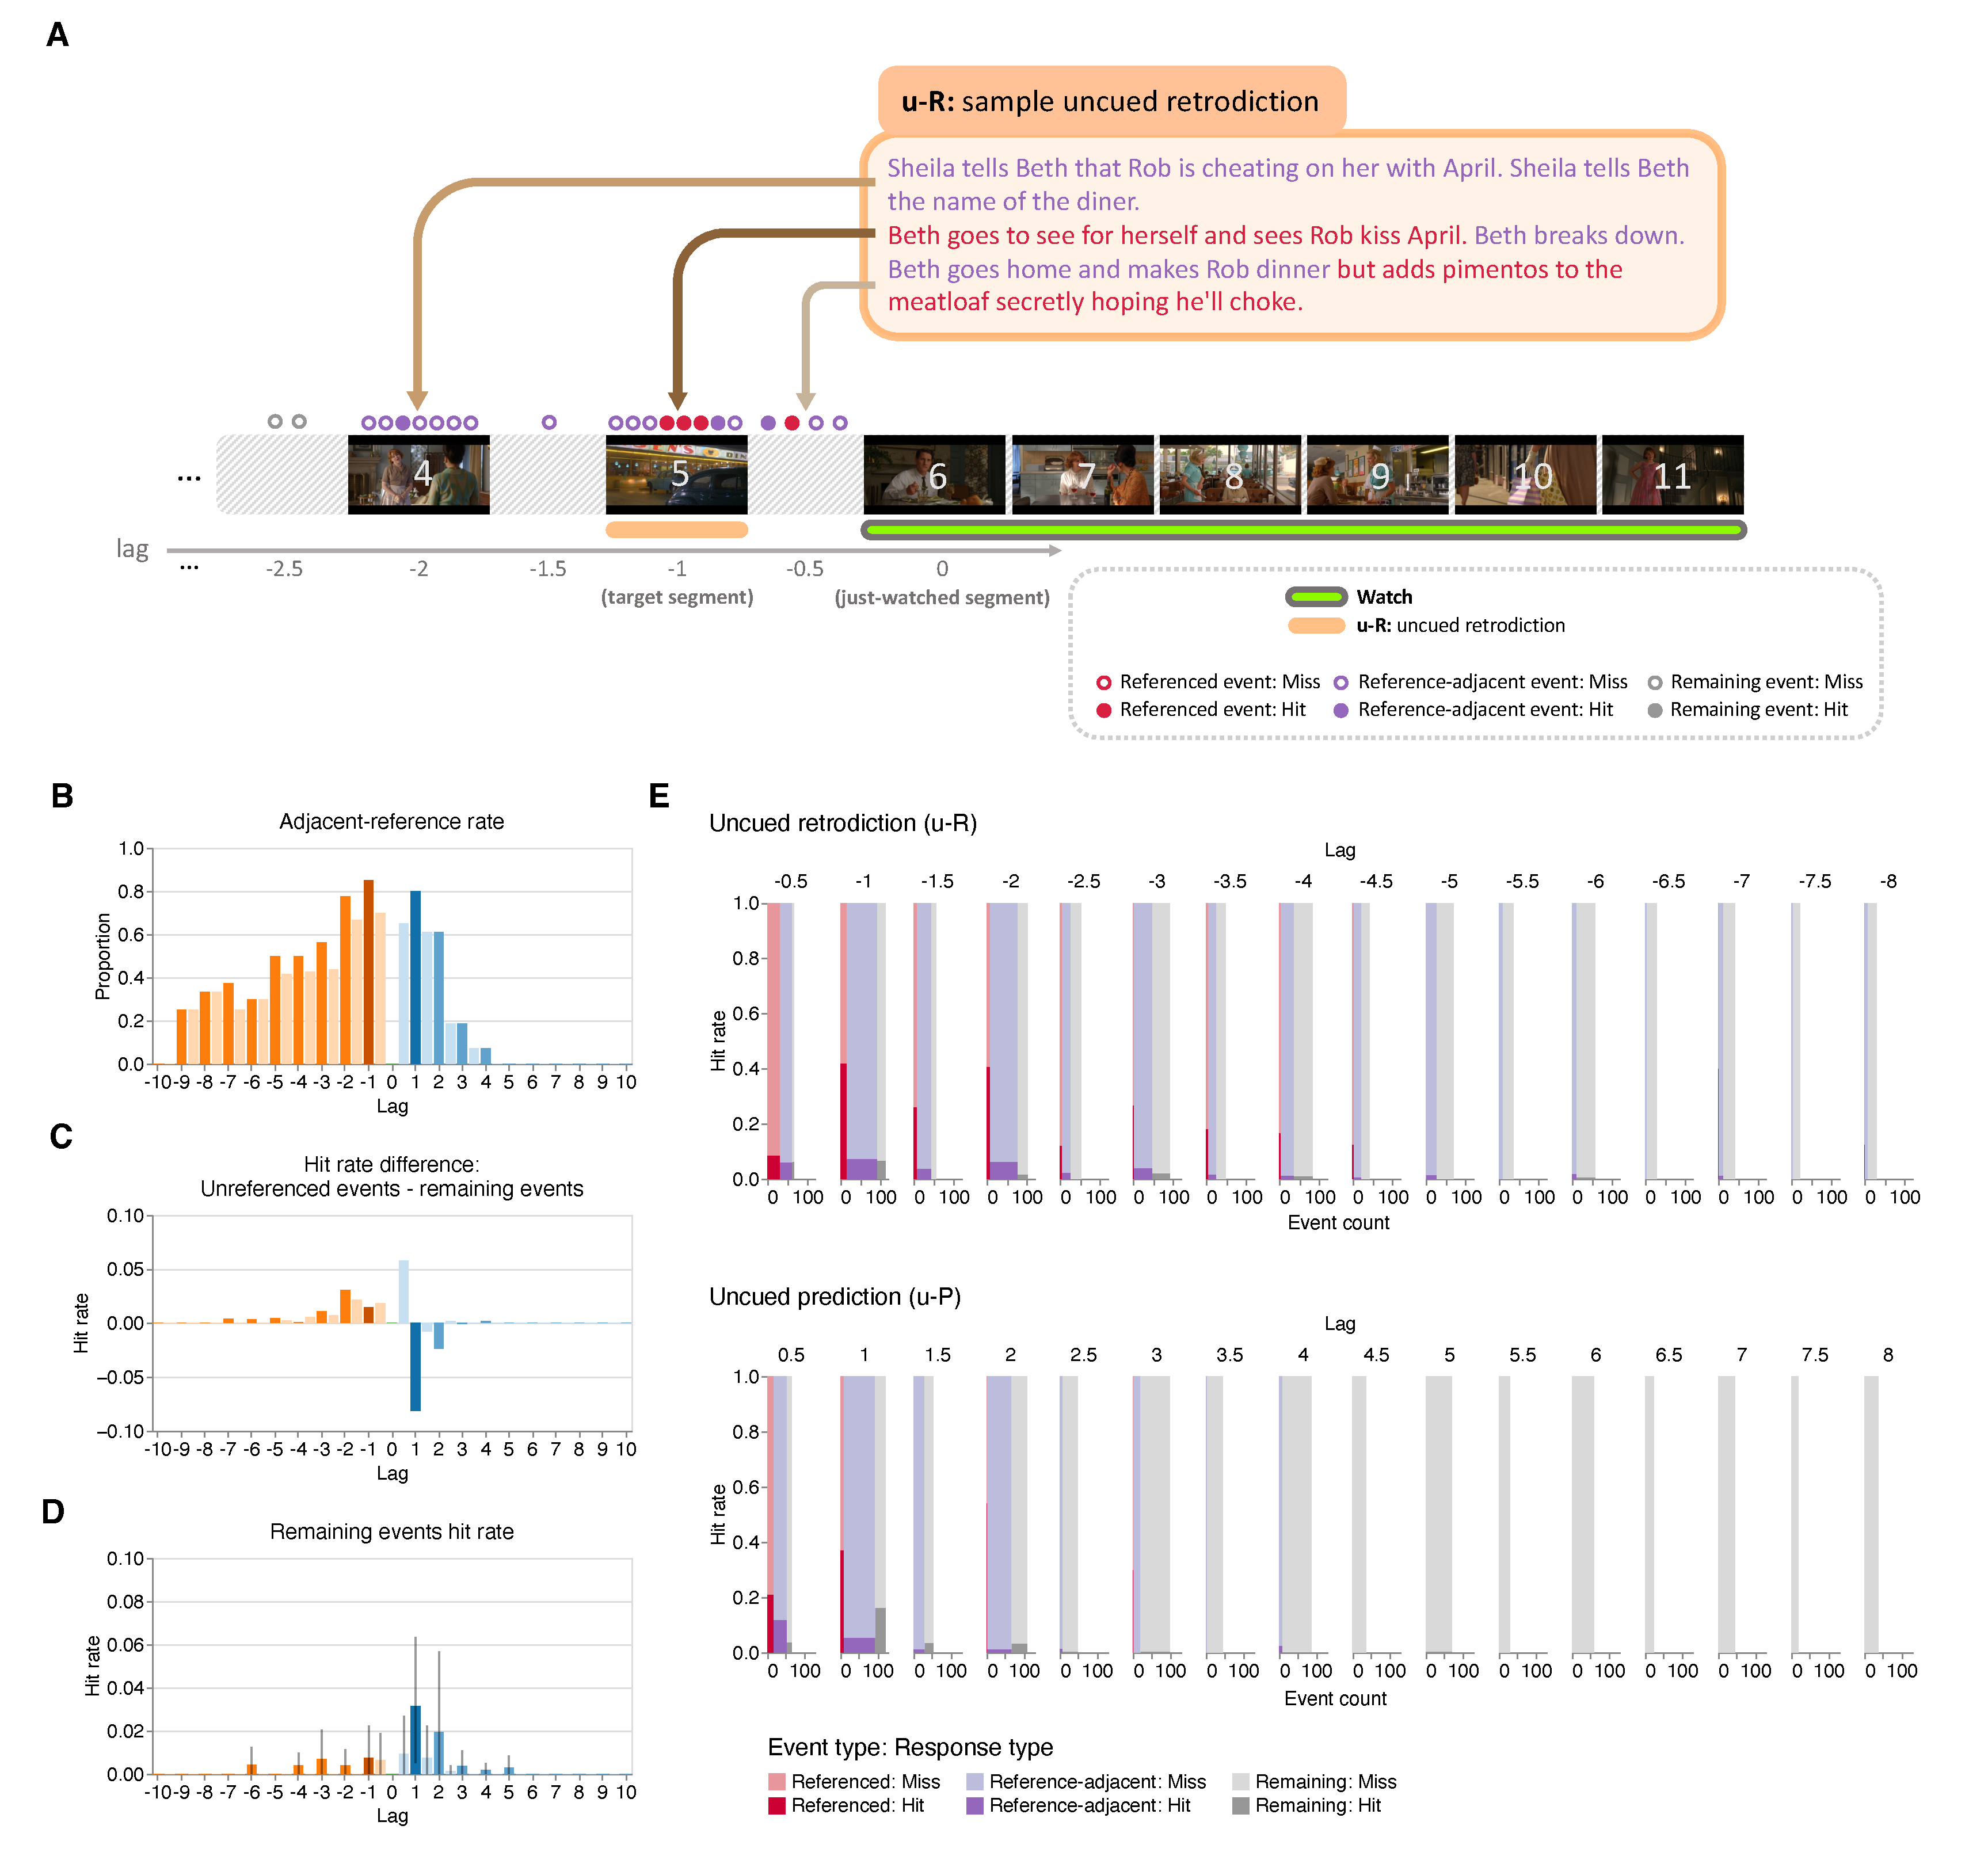
\includegraphics[width=0.8\textwidth]{results4}
  \caption{\textbf{Reference-adjacent events are associated with higher hit rates.}  \textbf{A. Illustration of annotation approach.}  We extended the annotation procedure depicted in Figure~\ref{fig:result3}A to also label unreferenced events that were either temporally adjacent to (i.e., immediately preceding or proceeding) a referenced event (reference-adjacent events) or not (remaining events).  \textbf{B. Adjacent reference rate for unreferenced events as a function of lag.}  Across all possible just-watched segments (lag 0), the bar heights denote the average proportion of unreferenced events in other past (orange, negative lags) or future (blue, positive lags) segments that were temporally adjacent to any referenced event.  \textbf{C. Difference in hit rates between unreferenced events and remaining events.}  To highlight the effect of reference adjacency on retrodiction and prediction of unreferenced events, here we display the difference in across-segment mean hit rates between unreferenced events and remaining events, as a function of temporal distance (lag) to the just-watched segment.  \textbf{D.  Hit rates for remaining events.}  The across-segment mean response hit rates for unreferenced events that were \textit{not} temporally adjacent to any referenced events are displayed as a function of temporal distance to the just-watched segment. Error bars denote bootstrapped 95\% confidence intervals.  Panels B--D: colors are described in the Figure~\ref{fig:result2} caption.  \textbf{E. Hit rates and counts of referenced, reference-adjacent, and remaining events.}  As a function of temporal distance to the just-watched segment, the sub-panels display the numbers ($x$-axes) and proportions ($y$-axes) of referenced (red), reference-adjacent (purple), and remaining (gray) events that participants hit (darker shading) or missed (lighter shading) in their uncued retrodictions (top sub-panel) and uncued predictions (bottom sub-panel).}
  \label{fig:result4}
\end{figure}

If characters' direct references cannot fully account for the temporal asymmetry in retrodicting the unobserved past versus predicting the unobserved future, what other factors might explain this phenomenon?  The results above indicate that characters’ references to specific unobserved events in the past or future boost participants’ estimates of these events.  If there are associations and dependencies between temporally adjacent events, might characters’ references to specific events also boost participants’ estimates of other events that were temporally \textit{adjacent} to the referenced events (Fig.~\ref{fig:result4}A)?  Because characters tended to refer to past events more often than future events, the proportions of unreferenced events that were adjacent to referenced events should show a similar temporal asymmetry in favor of the past.  We confirmed this intuition by computing the proportions of unreferenced events in the stimulus that were temporally adjacent to past or future events referenced by the characters during a given segment.  Here we defined \textit{temporally adjacent} as any event within an absolute lag of one relative to a referenced onscreen event, or within an absolute lag of 0.5 to a referenced offscreen event.  We also defined \textit{remaining} events as unreferenced events that were not temporally adjacent to any referenced events.  As shown in Figure~\ref{fig:result4}B, we observed higher proportions of unreferenced past than future events that were temporally adjacent to referenced events.  Further, these reference-adjacent events had higher hit rates than remaining events after controlling for absolute lag (uncued retrodiction: OR = 7.15, $Z = 2.40$, $p = 0.02$, CI: 1.44 to 35.58; uncued prediction: OR = 3.11, $Z = 2.30$, $p = 0.02$, CI: 1.18 to 8.21; Fig.~\ref{fig:result4}E).  To estimate the contributions of reference adjacency on hit rates, we computed the difference in hit rates between unreferenced events (which comprised both reference-adjacent and remaining events) and remaining events, as a function of lag.  These differences exhibited a temporal asymmetry in favor of retrodiction.  This suggests that reference-adjacent events also contribute to participants' retrodiction advantage.  Remaining events did \textit{not} exhibit a reliable temporal asymmetry (OR = 0.75, $Z = 0.33$, $p = 0.74$, CI: 0.14 to 4.08; Fig.~\ref{fig:result4}D), suggesting that, after accounting for temporal adjacency, character's references to past and future events can explain participants' retrodiction advantage.

\begin{figure}[tp]
  \centering
  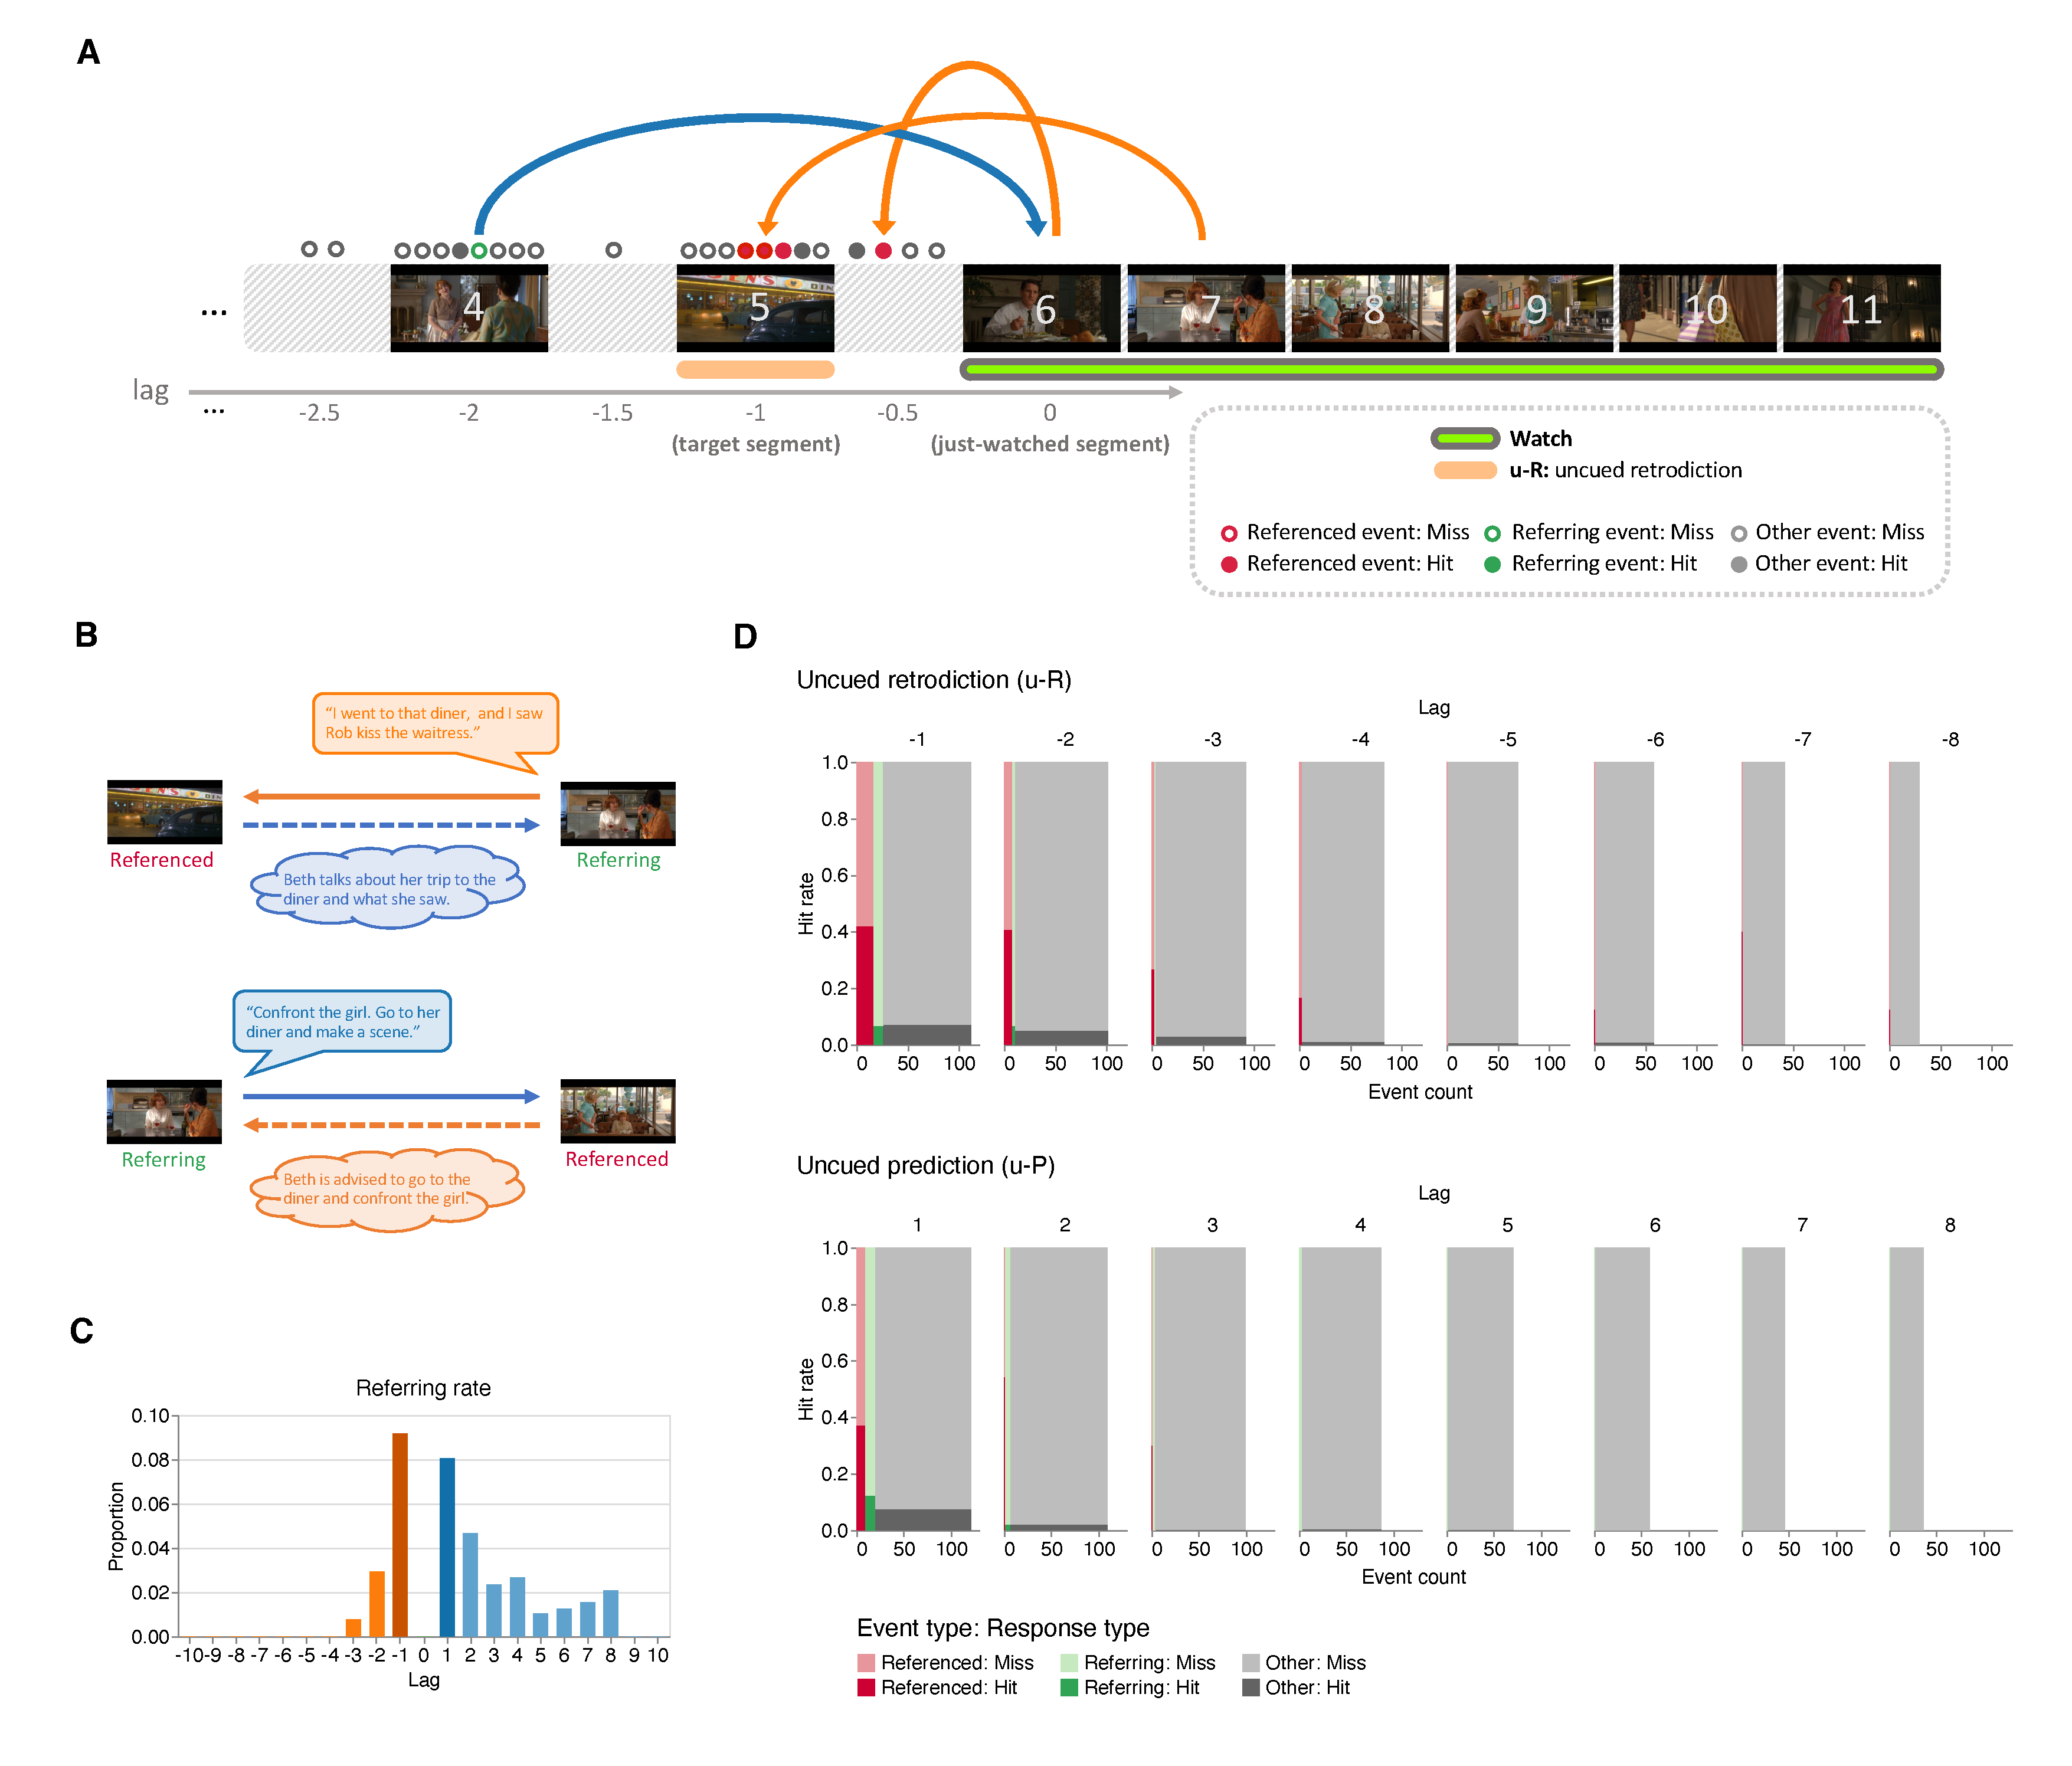
\includegraphics[width=\textwidth]{results5}
  \caption{\textbf{Referenced events are associated with higher hit rates, but referring events are not.}  \textbf{A. Illustration of annotation approach.}  We extended the annotation procedure depicted in Figure~\ref{fig:result3}A to also label which events \textit{contained} references to events in other segments.  \textbf{B. Referenced versus referring events.}  During event $i$, when a character makes a reference to another event ($j$), we define $i$ as the \textit{referring} event and $j$ as the \textit{referenced} event.  \textbf{C.  Referring rate as a function of lag.}  Across all possible just-watched segments (lag 0), the bar heights denote the across-segment mean proportions of events containing references to events in other past (orange, negative lags) or future (blue, positive lags) segments.  The bar colors are described in the Figure~\ref{fig:result2} caption.  \textbf{D. Hit rates and counts of referenced, referring, and other events.}  As a function of temporal distance to the just-watched segment, the sub-panels display the numbers ($x$-axes) and hit rates ($y$-axes) of referenced (red), referring (green), and other (gray) events that participants hit (darker shading) or missed (lighter shading) in their uncued retrodictions (top sub-panel) and uncued predictions (bottom sub-panel).}
  \label{fig:result5}
\end{figure}

The preceding analyses show that when characters reference past or future events, those referenced events, and other events that are temporally adjacent to the referenced events, are more likely to be retrodicted and predicted.  In other words, referring to a past or future event in conversation leads to a ``boost'' in that event's hit rate.  We wondered whether this boost was bi-directional.  In particular: when a character refers (during a \textit{referring event}) to another event (i.e., the \textit{referenced event}), does this boost only the referenced event's hit rate, or does the referring event also receive a boost?  We labeled each event as a ``referring event'', a ``referenced event'', or a ``other event'' (i.e., not referring or referenced; Fig.~\ref{fig:result5}A, B).  We limited our analysis to \DIFdelbegin \DIFdel{only references that referenced }\DIFdelend \DIFaddbegin \DIFadd{references to }\DIFaddend onscreen (explicit) events.   Consistent with our analysis of character's references to other events (Fig.~\ref{fig:result3}B), \textit{referring} events exhibited a \textit{forward} temporal asymmetry (Fig.~\ref{fig:result5}C).  Controlling for absolute lag, we found that referring events were associated with lower hit rates than referenced events (uncued retrodiction: OR = 0.03, $Z = -4.81$, $p < 0.001$, CI: 0.01 to 0.11; uncued prediction: OR = 0.04, $Z = -5.84$, $p < 0.001$, CI: 0.01 to 0.12; Fig.~\ref{fig:result3}D) and had no reliable differences in hit rates compared with other events (uncued retrodiction: OR = 0.37, $Z = -1.46$, $p = 0.15$, CI: 0.10 to 1.41; uncued prediction: OR = 2.16, $Z = 1.68$, $p = 0.09$, CI: 0.88 to 5.30).  This indicates that only referenced events received a hit rate boost (relative to referring events), suggesting that the retrodictive and predictive benefits of references are directed (i.e., asymmetric).


\section*{Discussion}
\DIFdelbegin \DIFdel{Associations across events form a complex web of interactions across a range of timescales that are characteristic of naturalistic stimuli and many real-world experiences.  The existence of across-event associations suggest that what is happening now is informative about what happened in the past and what might happen in the future.
}\DIFdelend While we have observations of our own past, the unobserved past in \textit{other} people's lives can seem as opaque as the not-yet-experienced future.  Here we used a character-driven television drama to test people's abilities to retrodict \DIFdelbegin \DIFdel{, predict, and remember}\DIFdelend \DIFaddbegin \DIFadd{the past and predict the future}\DIFaddend .  Our main finding is that participants tended to more accurately and more readily retrodict the unobserved past versus predict the unobserved future of the narrative.  We traced this temporal asymmetry to (a) characters' tendencies to refer to past events more than future plans in their ongoing conversations, and (b) associations between temporally proximal events (Fig.~\ref{fig:discussion}).  
\DIFdelbegin \DIFdel{Our work helps to reconcile the apparent discrepancy between the temporal symmetry posited by classical physics and the common subjective notion that we know more about the past than the future ~\mbox{%DIFAUXCMD
\citep{Cove94}}\hskip0pt%DIFAUXCMD
. 
In particular, when the present moment contains references to other moments in the past or future (e.g., as often occurs in natural conversations), this affects how we form inferences about the past and future. Our work also draws inspiration from prior related studies that suggest that our subjective experience of the ``present '' moment may be more accurately described as a blend of experiences spread over a wide range of times~\mbox{%DIFAUXCMD
\citep{Mann21a, MlodBrun14}}\hskip0pt%DIFAUXCMD
.
}\DIFdelend 

\begin{figure}[tp]
  \centering
  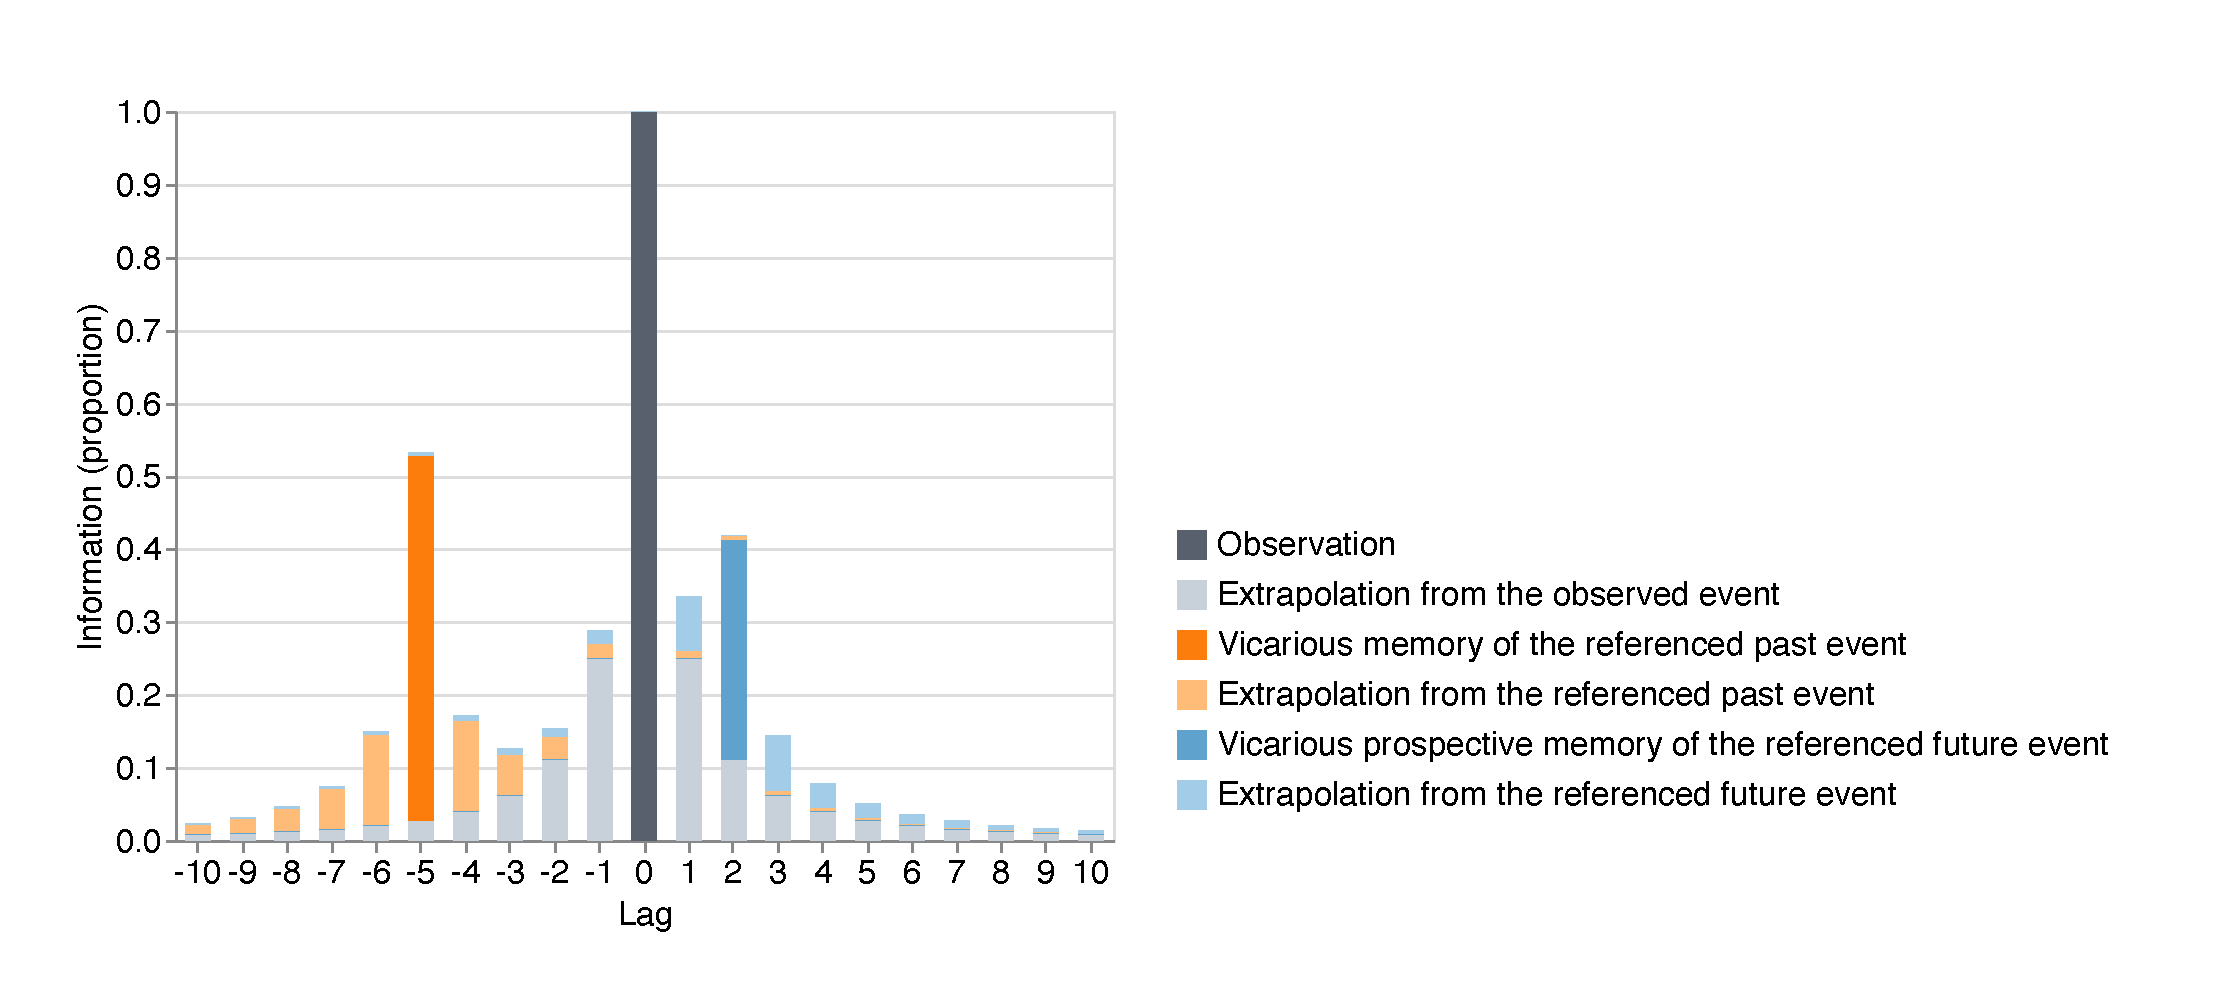
\includegraphics[width=\textwidth]{discussion}
  \caption{\textbf{How much information about the past and future can be extracted by observing the present?}  By definition, let us say that the present moment (lag 0) contains all information about itself (dark gray).  Given learned statistical regularities, one might extrapolate from the present moment into the past or future (light gray).  As illustrated in this schematic, the information contained in the present about other moments in time falls off with absolute lag.  This falloff is approximately time-symmetric.  References in the present to past events (dark orange) or future events (dark blue) provide additional information about those referenced moments in time, beyond what could be inferred solely from statistical regularities.  This additional information about those referenced moments can also be extrapolated to other moments that are temporally nearby to \textit{them} (light orange and blue).}
  \label{fig:discussion}
\end{figure}

\DIFaddbegin \DIFadd{While we have asymmetric knowledge about our own past and future, here we showed that in narrative events, we also have asymmetric knowledge about }\textit{\DIFadd{other people's}} \DIFadd{past and future from just observing the }\textit{\DIFadd{present}}\DIFadd{. 
Here, the present is in the form of a movie segment. What makes a movie segment different from time-symmetric Markov processes~\mbox{%DIFAUXCMD
\citep{Cove94}}\hskip0pt%DIFAUXCMD
? Our answer is that narrative events capture the notion that the present stores memories or traces of the past, but not of the future, while states in Markov processes are memoryless. 
}

\DIFaddend % role of conversational references
\DIFaddbegin \DIFadd{In the current study, memories or traces of the past were primarily expressed as references to past events in conversations between characters. Further, future plans could also be expressed in conversations, providing clues for what will happen in the future.
}\DIFaddend Previous work has recognized the conversational role of episodic memory and how conversation facilitates memory sharing~\citep{HirsEcht12, MahrCsib18, Dess07}.  This body of work suggests that, because people have memories of their own pasts, that knowledge can be transferred to third parties through conversation.  We extend this notion by showing that ``memory sharing'' need not be limited solely to past events.  Rather, conversations can also provide information about the future, in the form of shared prospective memories.  Our specific memories or prospective memories constrain what could have happened in our pasts or what might happen in our futures. Further, these memories or prospective memories could serve as anchor points that facilitate estimates of temporally adjacent events.

%DIF <  lies
\DIFdelbegin \DIFdel{While conversations can provide information about the unobserved past and/or future, it is important to recognize that the provided information may not be accurate.  For example, in the stimuli used in our study, we noted a total of 15 lies (referring to fake past or future events), and our participants occasionally retrodicted or predicted these lied-about events.  In general, the use of (known or unknown) lies as an information source about the unobserved past or future could provide useful insights into how we incorporate false information into our estimates.  On one hand, lies may mislead us.  On the other hand, lies might also contain usable information about unobserved events (e.g., about what might have happened in the past that could have led a character to tell a particular lie, etc.).
}%DIFDELCMD < 

%DIFDELCMD < %%%
%DIF <  boundary conditions
\DIFdelend %DIF >  boundary conditions and the differences between retrodicting/predicting narrative events and real-life events 
Although the stimulus our participants viewed contained more conversational references to the past than to the future~\citep[consistent with most real-world conversations;][]{DemiEtal18}, this bias towards the past is not reflective of \textit{every} conversation.  For example, a conversation about future plans, such as an upcoming vacation, might contain more references to the future than to the past.  Our work suggests that, in this example scenario, someone observing the conversation would be better at predicting the future than at retrodicting the past.  \DIFdelbegin \DIFdel{More generally, our tendency to better retrodict the past than predict the future is a reflection of the information that is typically available to us in the present moment, rather than a fundamental bias built into our memory systems themselves.
}%DIFDELCMD < 

%DIFDELCMD < %%%
%DIF <  difference between retrodicting/retrodicting narrative events and real-life events 
\DIFdel{Given that our study focused exclusively on narrative events, one could ask how retrodicting and predicting narrative events might differ from real-world retrodiction and prediction.  Narratives (including television shows, as in our study) are often carefully crafted to keep the audience engaged and entertained, and to compress the story duration to a convenient length.  Narrative techniques, such as foreshadowing, might provide the audience with information that is not typically available in real-world situations.  Another important difference between narratives }\DIFdelend \DIFaddbegin \DIFadd{However, when considering the differences between narrative }\DIFaddend versus real-world experiences\DIFaddbegin \DIFadd{, an important one }\DIFaddend is that narratives are typically observed passively whereas we typically play an active role in our real-world experiences.  A consequence is that the information we have (e.g., about the past or future) in a narrative is limited to what the writer provides to the audience.  In contrast, when we notice that we are missing information in real-world circumstances, we can often actively seek out what we are missing by interacting with other people, objects, and records.  In turn, this might affect how we retrodict or predict in narratives versus real-world circumstances.  For example, passively observing a conversation about the future (e.g., in a narrative) might inform us more about the future than the past.  But the ability to participate in that conversation (e.g., in a real-life situation) would give us potential access to the speaker's knowledge, which typically favors the past (e.g., Figs.~\ref{fig:intro1}, \ref{fig:intro2}).  
In principle, several aspects of our analysis and experimental paradigm could be adapted to study retrodiction and prediction of real-world events.  This could help to clarify the similarities and differences between these processes in narratives versus real-world circumstances.

%DIF >  belief and lies
\DIFaddbegin \DIFadd{While conversations contain asymmetric numbers of references to past and future events, for retrodictions to be better than predictions, it requires participants to actually believe in those references. Indeed, referenced events were associated with higher hit rates than unreferenced events, suggesting that participants did treat references as literal, either referring to past or future events. 
However, it is important to recognize that the provided information may not be accurate.  For example, in the stimuli used in our study, we noted a total of 15 lies (referring to fake past or future events), and our participants occasionally retrodicted or predicted these lied-about events.  In general, the use of (known or unknown) lies as an information source about the unobserved past or future could provide useful insights into how we incorporate false information into our estimates.  On one hand, lies may mislead us.  On the other hand, lies might also contain usable information about unobserved events (e.g., about what might have happened in the past that could have led a character to tell a particular lie, etc.).
}

%DIF >  why arrow of time
\DIFadd{One might ask why is there an arrow of time in real-life events, given that the fundamental laws of physics are time-reversible. Theoretically, if one is able to measure the position and velocity of every molecule in the universe (known as Laplace's demon), then one should be able to perfectly calculate the past state as well as the future state of every molecule (thus the universe), both of which are deterministic. 
We humans, with limited perception abilities, are not able to track every molecule in the world. Instead, we do coarse-graining on groups of microstates and describe macroscopic properties of the world.
Take the weather as an example, we typically use words like "cloudy" and "sunny" as macroscopic descriptions of the weather, instead of trying to describe the microstates of every molecule.
In statistical mechanics, the entropy of a macrostate is related to the number of microstates therein. 
The modern view is that one could make an assumption that the universe started in a low entropy state, known as the past hypothesis ~\mbox{%DIFAUXCMD
\citep{Albe00}}\hskip0pt%DIFAUXCMD
. Then, following the thermodynamic arrow of time, entropy will increase towards the future. In theory, there should be equal numbers of past and future trajectories that are compatible with the current macrostate. However, if adding the restriction that the past was in a lower entropy state, then we are able to rule out past trajectories that are not compatible with the past hypothesis, leaving us with less uncertainty, and thus more knowledge of the past, than the future~\mbox{%DIFAUXCMD
\citep{Carr10, Carr16}}\hskip0pt%DIFAUXCMD
. 
The past hypothesis might also explain why we have memories of the past, but not of the future. \mbox{%DIFAUXCMD
\cite{MlodBrun14} }\hskip0pt%DIFAUXCMD
showed that generically the psychological arrow of time should align with the thermodynamic arrow of time where the arrow is well defined~\mbox{%DIFAUXCMD
\cite[see also][]{Rove22}}\hskip0pt%DIFAUXCMD
. Thus, we can only remember the direction where entropy is lower, which we refer to as the past. However, this view is currently under debate~\mbox{%DIFAUXCMD
\citep{Golo21, HemmShen19}}\hskip0pt%DIFAUXCMD
.
}

\DIFadd{The past hypothesis could then be applied to the current study in two folds. One fold is that given that the psychological arrow of time aligns with the thermodynamic arrow of time, characters in the narrative would have memories of the past, and these memories could be expressed as references to past events in conversations. The other fold is that participants would assume a past hypothesis such that a past time point of the narrative story is of lower entropy than a future time point. The past hypothesis then help participants rule out possibilities of past events that incompatible with a lower entropy state. Specifically, participants would choose to believe characters' memories (as references to past events in conversations) and thus make correct retrodictions.
}

\DIFadd{One thing to note here is that unlike Markov processes where we can calculate the uncertainty of the past and the future given the present, for real-life events, there is no ground truth of the uncertainty, either of the past or the future. 
The notion of thermodynamic entropy is also subjective, as it depends on how we do coarse-graining, that is, how we group microstates into the same macrostate. 
In the current experiment, we measured the similarities/dissimilarities of people's retrodiction, predictions and recall of the narrative events. 
Another possibility is that the observed asymmetry in our knowledge about the past and future reflects 
the coarse-graining~\mbox{%DIFAUXCMD
\citep{Rove14} }\hskip0pt%DIFAUXCMD
in how we use language to describe events in either retrodictions, predictions, or recall. For example, when references aided retrodictions/predictions of the referenced events (Fig.~\ref{fig:result4}), in theory they should also aid retrodictions/predictions of the referring events. However, it was rare that participants would predict that characters will talk about (i.e., make a backward reference to) the current event. Future studies could use other measures to assess what we can infer about the past and the future given the present.
}

\DIFaddend % why retrodict
In our study, we explicitly designed participants' experiences such that both the past and future were unobserved.  How representative is this scenario of everyday life?  For example, we might try to speculate about the unobserved future when making plans or goals, but when might we encounter situations where the past is unobserved but still useful for us to speculate about?  
Real-life events have long-range dependencies.
In general, because the future depends on what happened in the past, discovering or estimating information about the unobserved past can help us form predictions about the future.  We illustrate this point in Figure~\ref{fig:discussion} by showing that the additional information contributed by a referenced past event can also extend into the future (light orange bars at lags $> 0$). 
This could explain why humans devote substantial effort and resources to attempting to figure out what happened in the unobserved past: history, anthropology, geology, detective and forensic science, and other related fields are each primarily focused on understanding, retrodicting, or reconstructing past events.   

\section*{Methods}
\subsection*{Participants}
A total of 36 participants (25 female, mean age 21.47 years, range 19--50 years) were recruited from the Dartmouth College community. All participants had self-reported normal or corrected-to-normal vision, hearing, and memory, and had not watched any episodes of \textit{Why Women Kill} before the experiment. Participants gave written consent to enroll in the study under a protocol approved by the Committee for the Protection of Human Subjects at Dartmouth College.  Participants received course credit or monetary compensation for their time. Two participants completed only the first half of the study and one participant’s data of the second half was lost due to technical error. All available data were used in the analyses.

\subsection*{Stimuli}
The stimulus used in the study were segments of the CBS television series \textit{Why Women Kill} Season 1. The TV series contained three distinct storylines depicting three women’s marital relationships. The three storylines, which took place in the 1960s, 1980s, and 2019, were shown in an interleaved fashion in the original episodes. The first 11 segments from the 1960s and 1980s storylines, across the first and second episodes, were used in our study. Segments were divided based on major scene cuts, which primarily corresponded to storyline shifts in the original episodes. The mean length of the segments was 2.05 min (range 0.97--3.87 min). We chose this TV series based on its strictly linear storytelling (within each storyline) and its realistic settings where most events depicted everyday life. The plots were focused on the main characters (Beth in storyline 1 and Simone in storyline 2), who were present in all the segments in the corresponding storylines.

\subsection*{Task design and procedure}
Our experimental paradigm was divided across two testing sessions. In each session, participants performed a sequence of tasks on segments from one storyline (Fig.~\ref{fig:method}).  For each storyline, there were four different task sequences: two forward chronological order sequences and two backward chronological order sequences. Participants completed one task sequence in forward chronological order for one storyline, and one in backward chronological order for the other storyline. The order of the two sessions (forward chronological order sequence first or backward chronological order sequence first), and the pairing of task sequences with storylines, were counterbalanced across participants.

Tasks in each sequence alternated between watching, recall, and retrodiction or prediction, with the specific order of tasks differing across the four sequences. For example, in sequence A1, participants first watched segment 1, followed by an immediate recall of segment 1. Then they predicted what would happen in segment 2 (first uncued and then character-cued). Participants then watched segment 3 and recalled segment 3. After that, participants guessed what happened in segment 2 again, which we termed ``updated prediction''. Then they watched segment 2, recalled segment 2, and so on as depicted in Figure~\ref{fig:method}.  This procedure was repeated to cover all possible segments.
We also note several edge cases at the start and end of the narrative sequences.  Since no segments precede the first segment, participants could never make ``prediction'' responses with the first segment as their target.  For analogous reasons, participants never made ``retrodiction'' responses with the last segment as their target.  Another edge case occurred in task sequences B2 and A2 (Fig.~\ref{fig:method}).  In the A1 and A2 sequences, participants experience the narrative in the original (forward) order, predicting one segment ahead along the way.  In the B1 and B2 sequences, participants experience the narrative in the reverse order, retrodicting one segment ahead along the way.  However, because A2 and B2 are offset from A1 and B2 by one segment, the initial A2 responses are \textit{retro}dictions, and the initial B2 responses are \textit{pre}dictions (i.e., they conflict with the temporal directions of the remaining responses in those conditions).  We therefore excluded from our analysis those initial retrodiction responses from the A2 condition, and the initial prediction responses from the B2 condition.

Before watching each segment, participants were given the following task instructions. After watching the video, participants were instructed to type their responses (retrodiction, prediction, or recall) in 1--4 sentences.  Participants were also asked to specify the characters' names in their responses, i.e., avoiding use of characters' pronouns. For the recall task, the names of the characters in the recall segment were displayed, and participants were asked to summarize the major plot points in the present tense. For the retrodiction and prediction tasks, participants were instructed to retrodict or predict the major plot points of the segment (also in the present tense), as though they had watched the segment and were writing a plot synopsis. They were also instructed to avoid speculation words (e.g., ``I \textit{think} Beth will...''). For the uncued retrodiction and prediction tasks, participants made retrodictions or predictions without any cues provided, so they had to guess which of the characters would be present in the segment. For character-cued retrodictions and predictions, the characters in the target segment were revealed on the screen, alongside participants’ previous responses. Participants were instructed to include or incorporate those characters into their character-cued responses, if their previous responses did not contain all the characters provided. They were also told that the characters were not necessarily listed in their order of appearance in the segment, and that only the main characters would be given. Also, the characters given did not necessarily interact with each other in that segment, and they could appear in successive events in that segment. If participants’ previous responses included all the characters given, then they could directly proceed to the next task without updating their response. For all of the prediction and retrodiction tasks, participants were instructed to provide at least one response, but they were given the opportunity enter up to three responses if they felt that multiple possibilities were more or less equally likely. Each response (including recall) was followed by a confidence rating on a 1--5 point scale. However, these confidence data were not analyzed in the present study.

Before their first testing session, participants were given a practice session, where they watched the first segment of storyline 3 followed by a recall trial, an uncued prediction trial, and a character-cued prediction trial. Participants' responses were checked by the experimenter to ensure compliance with the instructions. To provide participants with sufficient background information about the storyline (especially for the backward chronological sequences), at the beginning of each session, participants were shown the time, location, and the main characters (with pictures) of the storyline. The first session was approximately 1.5~h long and the second session was approximately 1~h long. We allowed participants, at their own discretion and convenience, to sign up for two consecutive testing time-slots (i.e., with their testing sessions occurring in immediate succession), or for testing sessions on two different days. The mean inter-session interval was 0.73 days (range: 0--4 days). The experiment was conducted in a sound- and light-attenuated testing room. Videos were displayed using a 27-inch iMac desktop computer (resolution: $5120 \times 2880$) and sound was presented using the iMac’s built-in speakers. The experiment was implemented using jsPsych~\citep{deLe15} and JATOS~\citep{LangEtal15}.

\subsection*{Video annotation}
Events in the first 11 segments of the two storylines were identified by the first author (X.X.), corresponding to major plot points (total: 117; mean: 5.32 per segment; range 3--9). Additionally, 74 offscreen events were identified. Of these 74 offscreen events, 43 events were identified from references in conversations during onscreen events. Another 16 events were identified based on characters’ transits between two places.  For example, if in segment 1 character A was in place A and in segment 2 she was in place B, then the transit from place A to B for character A would be identified as an offscreen event. The remaining 15 offscreen events were identified based on logical inferences.  For example, if a photo was shown in an onscreen event (but not the act of it being taken), then the action that someone took the photo would be identified as an offscreen event.  Offscreen events always occurred between two contiguous segments, or before the first segment. The purpose of identifying offscreen events was to match participants’ responses to video events; thus our identification of these offscreen events was not intended to be exhaustive.

\subsection*{Response analyses}
Participants' retrodiction, prediction, and recall responses were minimally processed to correct obvious typos (e.g., in characters’ names) and remove speculation descriptions (e.g., ``I predict that...'').  All responses were manually coded and matched to events from the video annotations. Retrodiction and prediction responses were coded by two coders (X.X. and Z.Z.). Recall responses were coded by one coder (X.X.).  While most responses were clearly identifiable as either matching specific storyline events or as not matching any storyline events, several ambiguous cases arose.  First, some responses combined or summarized over several (distinct) storyline events.  Second, some responses lacked any specific detail (e.g., ``character A and B talk'' without describing the specific topic(s) of conversation or providing other relevant details).  Based on participants' responses, in addition to the original 117 onscreen events and 74 offscreen events, we added 25 new events (23 onscreen, 2 offscreen) that either summarized across several events or partially matched the annotated events.  Whereas the original events were each assigned a value of one point, we assigned these additional events a half point.  This point system enabled us to directly match events in participants' responses to the annotated events.  In our analyses of retrodictions, predictions, and recalls, we added up the number of points earned for each response to estimate participants' event hit rates.

We coded only the first retrodiction or prediction response in each trial.  For these responses, we also only considered storyline events that were in the same temporal direction as the target segment.  For example, if a participant was asked to retrodict what happened in segment $n$, only events from segments $1...n$ were considered in our analysis.  When coding recall responses, we considered only events from the target segment.  

An additional ambiguous case arose in one participant's responses pertaining to segment 12, storyline 2, whereby the participant correctly identified an onscreen event that had not been included in our original annotations.  To account for this participant's response, we retroactively added that event to our annotations of that segment.  We also identified and counted unmatched events in participants' responses (i.e., events that did not match any annotated events).  In several cases, the two coders' independent scoring disagreed.  These cases were resolved through discussions between the two coders.

To estimate the semantic similarities between pairs of responses, we first transformed each response into a 512-dimensional vector (embedding) using \textit{Universal Sentence Encoder}~\citep[Transformer USE, ][]{CerEtal18}.  We defined \textit{similarity} as the cosine of the angle formed by the responses' vectors.  Following~\cite{HeusEtal21}, we defined the \textit{precision} of participants' responses as the median similarity between that response's vector and the embedding vectors for all other participants' recalls of the target segment.  We defined the \textit{convergence} of a given response as the mean similarity between that response's vector and all other participants' responses to the corresponding segment, in the same condition.  To compute these median or mean similarities we first applied the Fisher $z$-transformation to the similarity values, then took the median or mean of the $z$-transformed similarities, and finally applied the inverse $z$-transformation to obtain the precision or convergence score.

To test the validity and reliability of the USE embeddings, we performed a classification analysis of recall responses using a leave-one-out approach. For each recall response, we calculated its semantic similarity with all other recall responses for the same storyline.  We took the segment with the highest median semantic similarity (to the recall response) as the ``predicted'' segment.  Across all responses, the predicted segments matched the true recalled segments' labels 98.6\% of the time (1088 out of 1103 predictions; chance level: 9\%).

\subsection*{Reference coding}
Two coders (X.X. and Z.Z.) identified character dialogues in the narrative that referred to past events or future (onscreen or offscreen) events.  Only references to events that occurred in a different segment were included in this tagging procedure.  For each reference, the source segment and the referred event number were recorded. A total of 82 references were identified.  Of these, 30 referred to onscreen events and 52 referred to offscreen events. For these referenced events, their corresponding summary events or partial events were also labelled as referenced. In instances where the coders disagreed about a given tag, disagreements were resolved through discussions between the two coders.  In our analyses, each storyline event was coded according to whether or not it had been referenced in the segment(s) that the participant had viewed thus far in the experiment.

In principle, a given event could receive multiple labels.  For example, during event $A$, a character might speak about another event, $B$, during which a reference to a third event ($C$) was made.  In this scenario, event $B$ could be both a ``referring event'' ($B \rightarrow C$) \textit{and} a referenced event ($A \rightarrow B$).  In practice, however, this scenario was quite rare, accounting for only one out of a total of 30 onscreen events.

\subsection*{Statistical analysis}
We used (generalized) linear mixed models to analyze the hit rates and numbers of events retrodicted, predicted, and recalled, as well as the precisions and convergences of participant's responses.  Our models were implemented in \texttt{R} using the \texttt{afex} package.  We carried out comparisons or contrasts, and extracted $p$-values, using the \texttt{emmeans} package.  Participants and stimuli (e.g., segment identity) were modeled as crossed random effects (as specified below).  Random effects were selected as the maximal structure that allowed model convergence. All of our statistical tests were two-sided.

For our tests of the target event hit rates across four \texttt{levels} (uncued, character-cued, updated, and recall; Fig.~\ref{fig:result1}B), we fit a generalized linear mixed model with a binomial link function:
\begin{lstlisting}[language=R]
  cbind(thp, ttp - thp) ~ direction * level * seg_cnt * storyline +
(direction * level | target) +
(direction * level * seg_cnt | subject)
\end{lstlisting}
where \texttt{thp} was the number of points hit for the target segment, \texttt{ttp} was the total number of points for the target segment (from its annotations), \texttt{direction} was either retrodiction or prediction, \texttt{level} had four levels (uncued, character-cued, updated, and recall), \texttt{seg\_cnt} represented the number of segments in the storyline that had been watched (1--10, centered),  \texttt{storyline} had two levels (1 or 2), and \texttt{target} had 22 levels according to the identity of the target segment.  For our tests of precision and convergence (Fig.~\ref{fig:result1}C, D), we fit linear mixed models using the same formula.  To test the effect of \texttt{direction} (retrodiction or prediction) on target event hit rates, precision, and convergence, we fit a (generalized) linear mixed model separately for each of the three levels (uncued, character-cued, and recall).  

For our tests comparing the numbers of hits for different types of events (Fig.~\ref{fig:result2}B), we fit generalized linear mixed models using the same formula, but with a poisson link function.  For these models, we manually doubled the point counts to ensure that half points were mapped onto integers, ensuring compatibility with the poisson link function.

For our analyses of the numbers of events hit, controlling for lag (Fig.~\ref{fig:result2}C), we fit a generalized linear mixed model with a poisson link function:
\begin{lstlisting}[language=R]
  hp_lag ~ direction * full_stp * lag * storyline +
  (direction | base_seg) + (1 | base_seg_pair) +
  (direction * full_stp | lag * storyline | subject)
  
\end{lstlisting}
where \texttt{hp\_lag} is the numbers of ``points'' earned (for each lag) in each trial (we manually doubled the point counts to ensure that half points were mapped onto integers, for compatibility with the poisson link function), \texttt{full\_stp} denoted whether the given events (of the given lag) were onscreen (i.e., full step) or offscreen (i.e., half step), \texttt{lag} denotes the (centered) absolute lag, \texttt{base\_seg} denotes the identity of the just-watched segment (22 levels), and \texttt{base\_seg\_pair} denotes the pairing of the just-watched segment and the segment at each lag (440 levels).

For our analyses of the proportions of events hit for referenced versus unreferenced events (Fig.~\ref{fig:result3}D, E), we fit a generalized linear model with a binomial link function:
\begin{lstlisting}[language=R]
  cbind(hp_lag, tp_lag - hp_lag) ~ direction * reference * full_stp +
  lag + (direction | base_seg) +
  (1 | base_seg_pair) +
  (direction * reference * full_stp + lag | subject)
\end{lstlisting}
where \texttt{hp\_lag} denotes the number of earned hit points for each reference type (referenced or unreferenced) at each lag, \texttt{tp\_lag} denotes the total number of possible hit points for each reference type at each lag, and the other variables adhered to the same notation used in the above formulas.

For our tests of the proportions of events hit for all three reference types (referenced, reference-adjacent, and remaining: Fig.~\ref{fig:result4}D, E; or referenced, referring, and other: Fig.~\ref{fig:result5}D), we fit a generalized linear mixed model using the same formula as above, but with three (rather than two) \texttt{reference} levels.

\section*{Code and data availability}
All of the code and data generated for the current manuscript are available online at:

https://github.com/ContextLab/prediction-retrodiction-paper

% \bibliographystyle{apa}
\DIFdelbegin %DIFDELCMD < \bibliography{CDL-bibliography/cdl}
%DIFDELCMD < %%%
\DIFdelend \DIFaddbegin \bibliography{CDL-bibliography/cdl, CDL-bibliography/temp}
\DIFaddend 

\section*{Acknowledgements}
We thank Luke Chang, Yi Fang, Paxton Fitzpatrick, Caroline Lee, Meghan Meyer, Lucy Owen, and Kirsten Ziman for feedback and scientific discussions.  Our work was supported in part by NSF CAREER Award Number 2145172 to J.R.M. The content is solely the responsibility of the authors and does not necessarily represent the official views of our supporting organizations.  The funders had no role in study design, data collection and analysis, decision to publish, or preparation of the manuscript.

\section*{Author contributions}
Conceptualization: X.X. and J.R.M.; Methodology: X.X. and J.R.M.; Software: X.X.; Analysis: X.X. and Z.Z.; Writing, Reviewing, and Editing: X.X., Z.Z., and J.R.M.; Supervision: J.R.M.

\section*{Competing interests}
The authors declare no competing interests.
\end{document} 